
\section{Resümee}


\section{Anhang}

\subsection{Abmessungen (BSVN)}


\begin{figure}[H]
    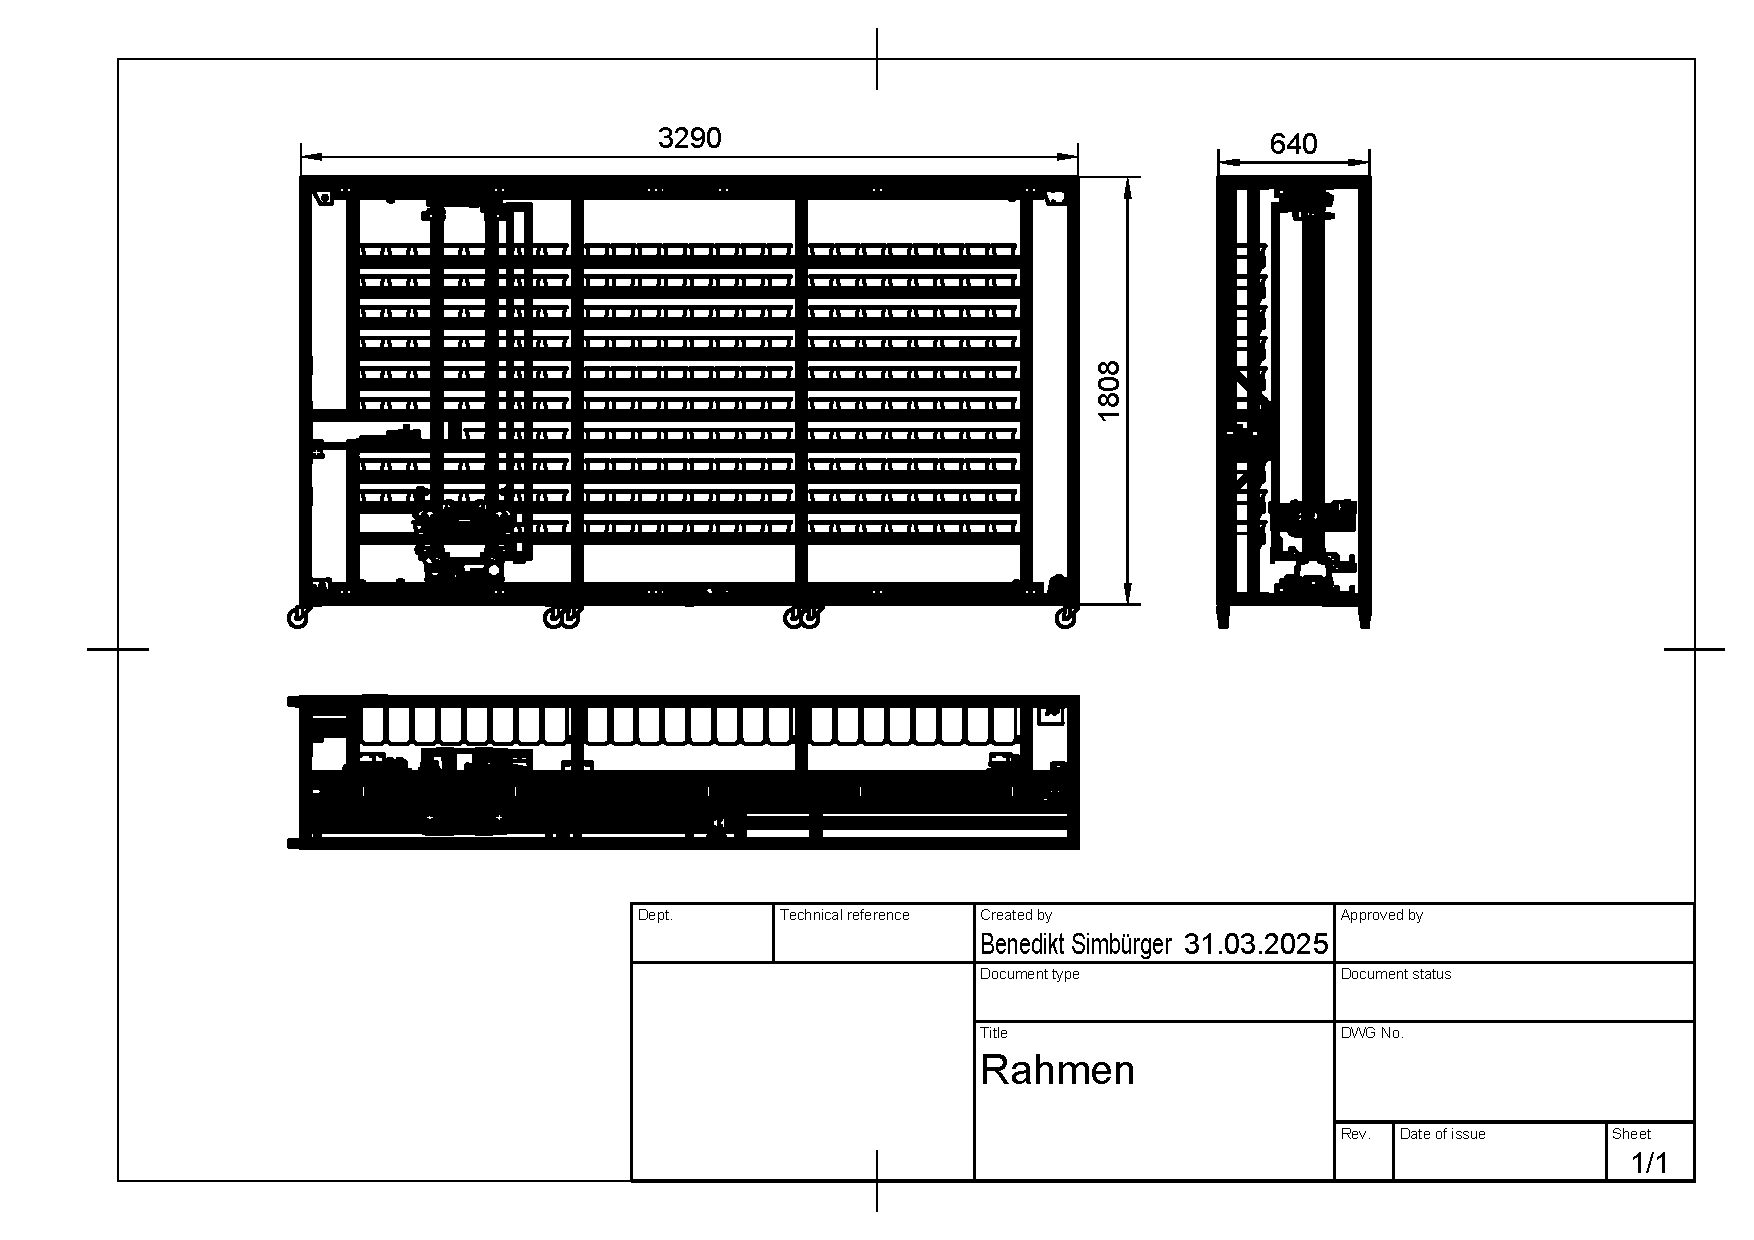
\includegraphics[width=\textwidth]{abmessungen_rahmen.pdf}
    \centering
    \caption{Abmessungen Rahmen}
\end{figure}
\begin{figure}[H]
    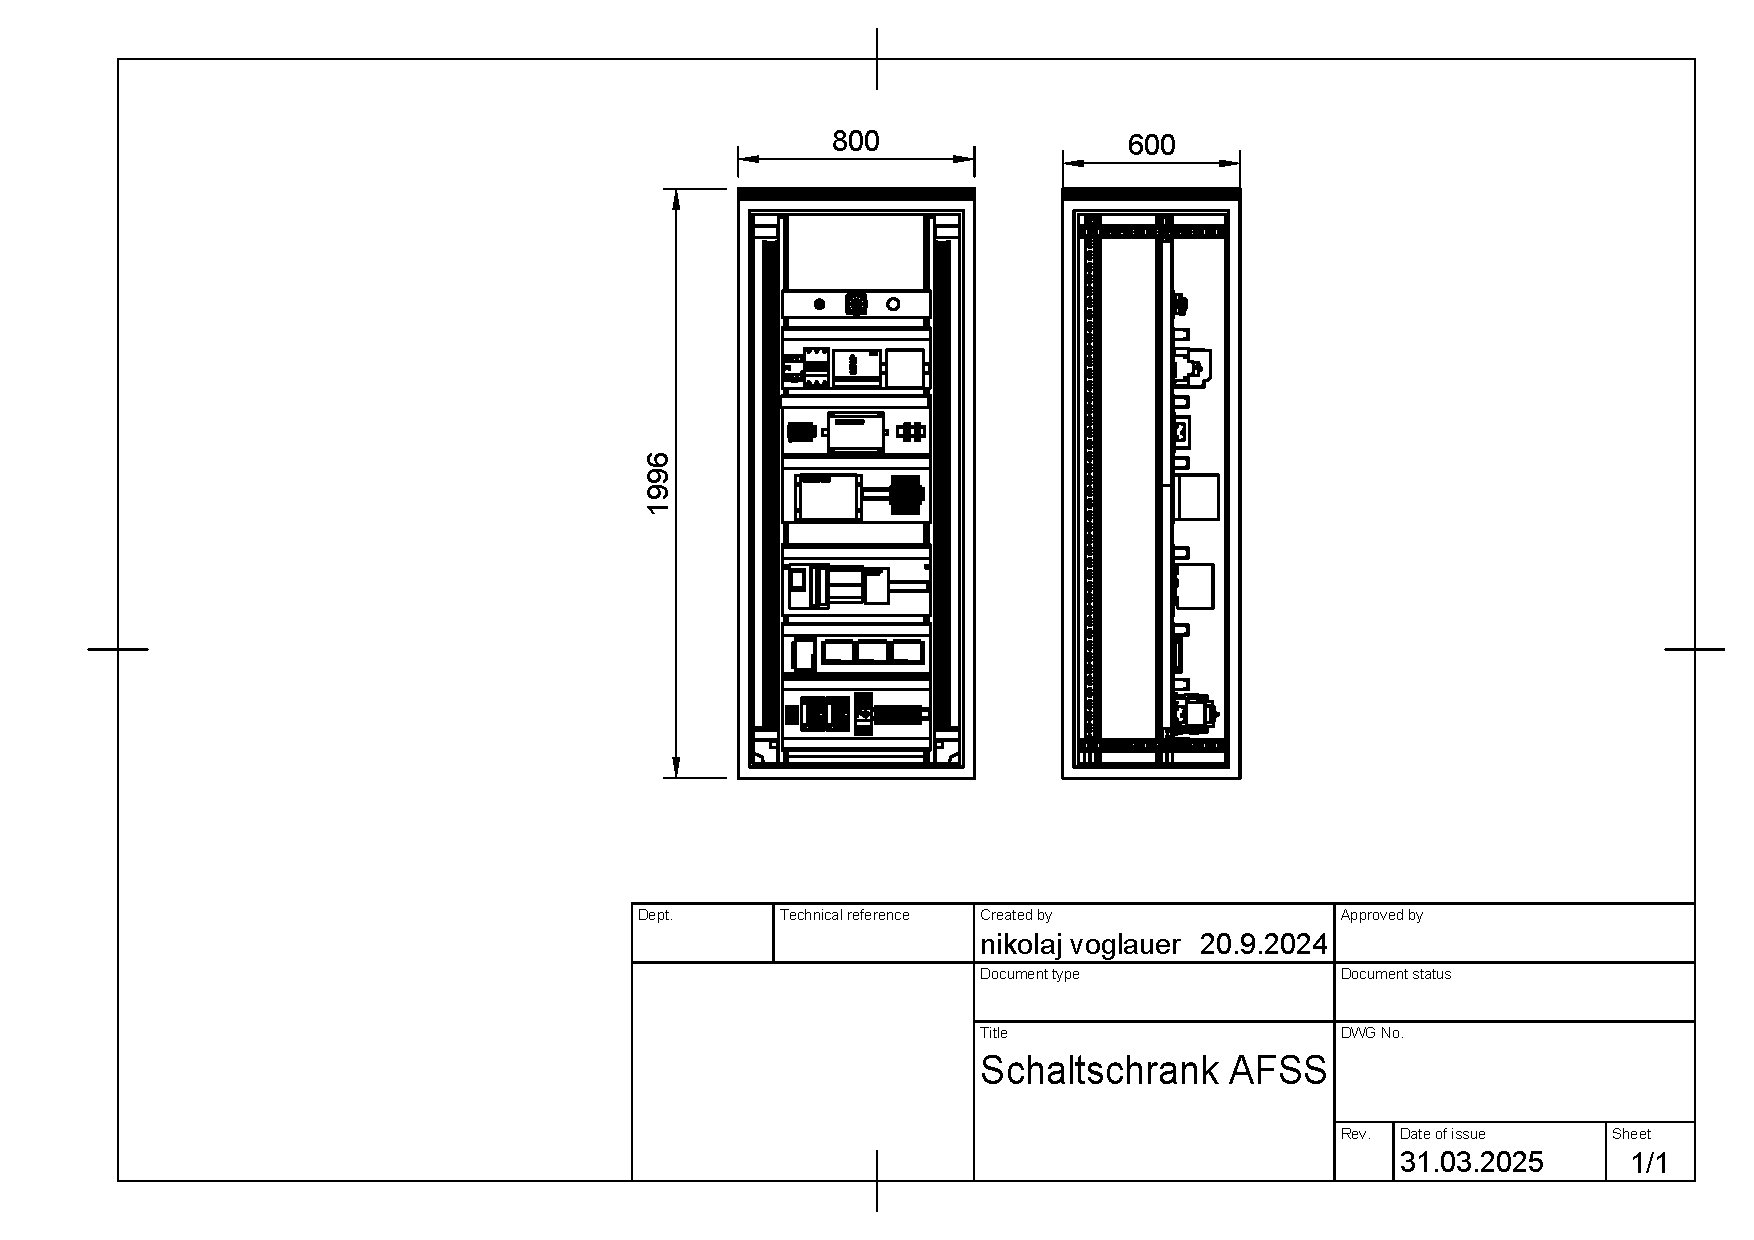
\includegraphics[width=\textwidth]{Vogis Bilder/Maximaldaten.pdf}
    \centering
    \caption{Abmessungen Rahmen}
\end{figure}

\subsection{E-Plan}

\subsection{Projektmanagement}
In diesem Kapitel wird auf das Projektmanagement des AFSS eingegangen. Dieses umfasst die zu Beginn des Projekts ausgearbeitete Aufgabenstellung und die einzelnen Arbeitspakete der jeweiligen Schülerin und Schüler. Außerdem wurde ein Produktstrukturplan angefertigt, in dem die Teilbereiche des Projekts und dessen zuständige Schülerin oder Schüler erkennbar ist. Ein weiterer Teil es Projektmanagements ist der Projektstrukturplan, welcher die unterschiedlichen Arbeitsschritte des Projekts veranschaulicht. Dieses Kapitel beinhaltet auch die in MS Project angefertigte Terminplanung.

\subsubsection{Aufgabenstellung des Gesamtprojekts}
\paragraph{Ausgangslage}\mbox{}\\
Die Werkstätte hat ein bestehendes Lager für Bauteile, die von Fachlehrern bestellt werden können. Jene Bestellungen werden dann von Schülerinnen und Schüler zusammengestellt und geliefert. Die Verwaltung dieses Lagers gestaltet sich allerdings schwierig, da Schülerinnen und Schüler beim manuellen Ein- und Auslagern z.B. den Lagerplatz vertauschen und es zu Fehlern kommt.

\paragraph{Untersuchungsanliegen der individuellen Themenstellungen}\mbox{}\\
Das Hauptanliegen dieser Diplomarbeit ist es, eine Anlage zu entwickeln, errichten und in Betrieb zu nehmen. Das bestehende System, mit manueller Handhabung, ist aufgrund des stetigen Bedienerwechsels sowie deren Ungenauigkeit, fehleranfällig. Der dadurch entstehende Mehraufwand verbraucht zusätzliche Ressourcen des Lehrpersonals. Um das Lehrpersonal sowie die Schülerinnen und Schüler zu entlasten, soll hier eine automatisierte Lösung entstehen. Es soll erwogen werden, welche Lösungen nötig sind, um ein Produkt zu planen und zu bauen, sodass dieses auch von nachfolgenden Schülerinnen und Schülern für zukünftige Anforderungen erweitert werden kann. Auch die Schnittstellen zwischen Hardware und Software, sowie die Ansteuerung der Mechanik soll in diesem Rahmen untersucht werden. Zudem soll die Sicherheit der Benutzerinnen und Benutzer immer gewährleistet sein.\\
\textbf{Simbürger Benedikt:} Programmierung des Backend und Hardwareentwicklung\\
\textbf{Sonvilla Vincent:} SPS-Programmierung und Serverkommunikation\\
\textbf{Voglauer Nikolaj:} Schaltschrankbau und Verkabelung sowie Hardwareentwicklung für Querförderer und Förderband\\
\textbf{Widmann Elena:} Auslegen elektrischen Komponenten, Ansteuerungen über Bussysteme und Sicherheitskonzeptionierung

\paragraph{Zielsetzung}\mbox{}\\
Erstellung einer Anlage, welche automatisch die gewünschte Ware mittels eines dreiachsigen Roboters, bereitstellt. Über eine Website soll eine Bestellung eingereicht werden können und der Server soll dann mit der SPS kommunizieren. Die Anlage lagert die Bestellung aus und nach Gebrauch wieder ein. Das effiziente Lagersystem soll ein hochtechnisiertes Vorzeigeprojekt der Schule werden.

\paragraph{Geplantes Ergebnis der individuellen Themenstellungen}\mbox{}\\
Die vom Benutzer gewünschten Bauteile werden aus einem Lagerplatz zu einer Kommissionier-Station gebracht und wieder zurückgestellt. Zum Herausheben der Bauteile, welche sich in Boxen befinden, ist ein vertikal montierter Portalroboter, an welchem eine Gabel montiert ist, verbaut. Ein Querförderer schiebt die angeforderten Boxen zwischen einem Förderband, welches die Boxen zum Endkunden befördert, und dem Lagersystem hin- und her. Die Bestellung ist über einen Web-Server möglich, welcher mit einer SPS kommuniziert.

\subsubsection{Produktstrukturplan}
\vspace{5mm}

\bgroup
    \centering
    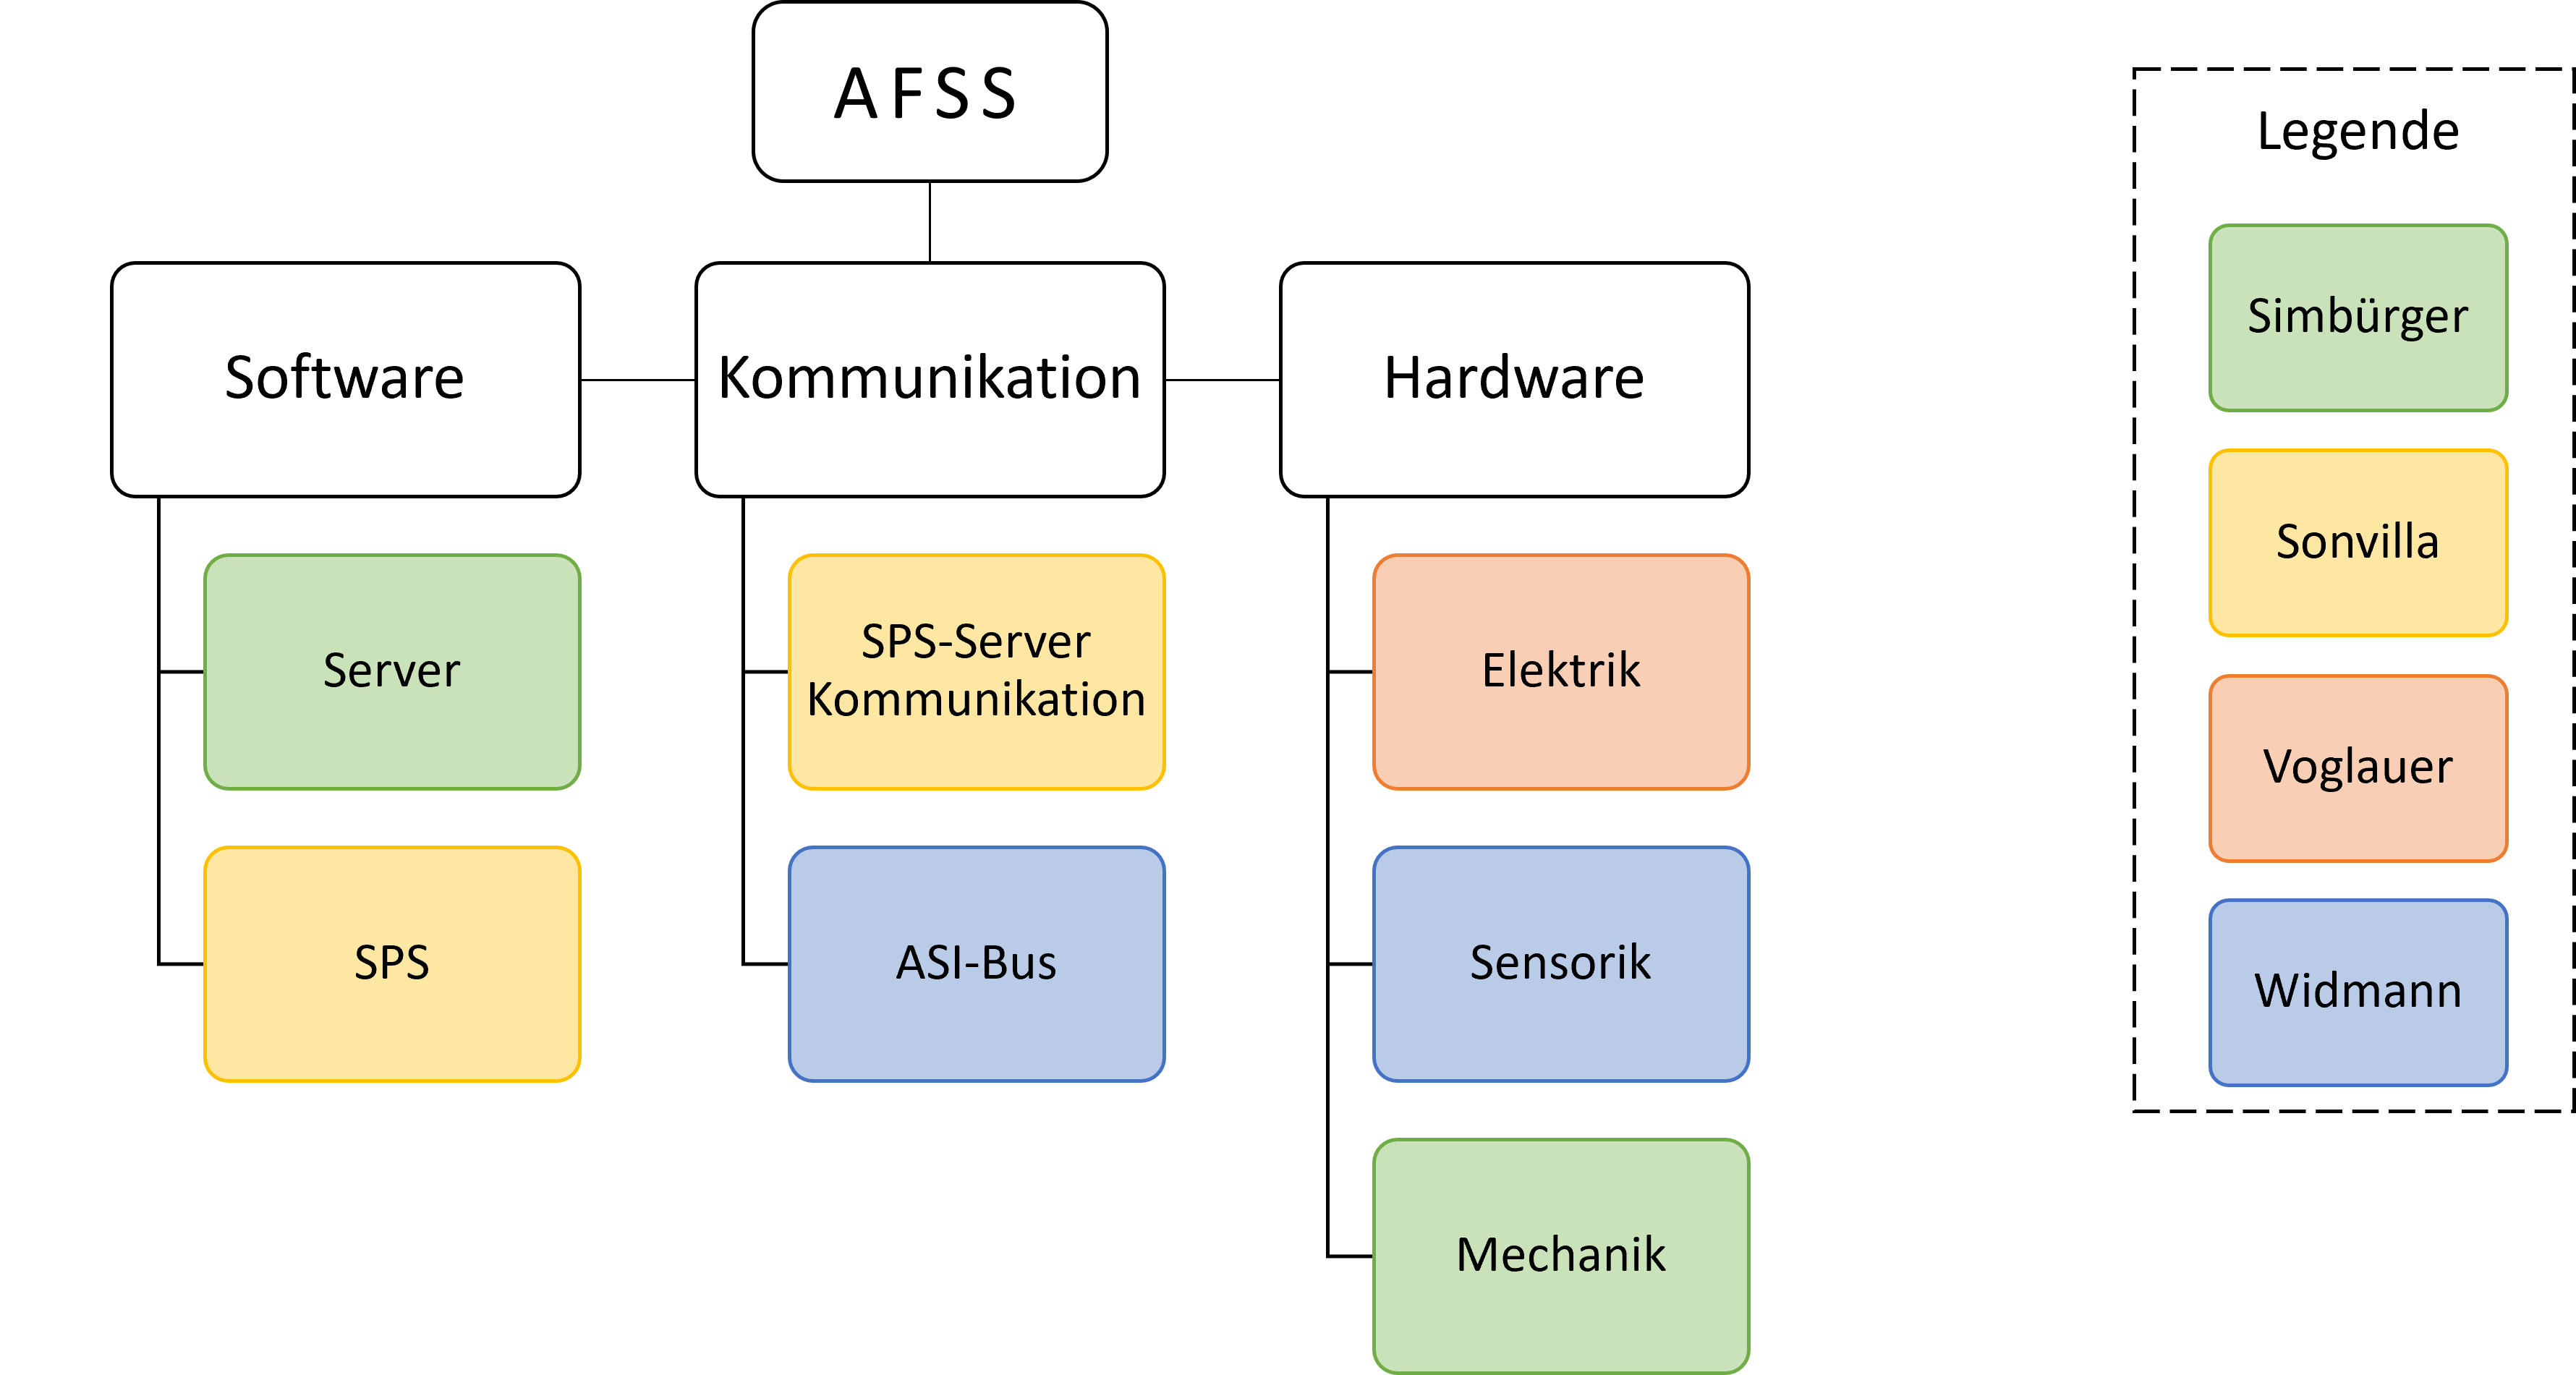
\includegraphics[width=0.9\textwidth]{WorkBreakdownStructure.png}
    \captionof{figure}{Produktstrukturplan}
\egroup

\subsubsection{Projektstrukturplan}
\vspace{5mm}

\bgroup
    \centering
    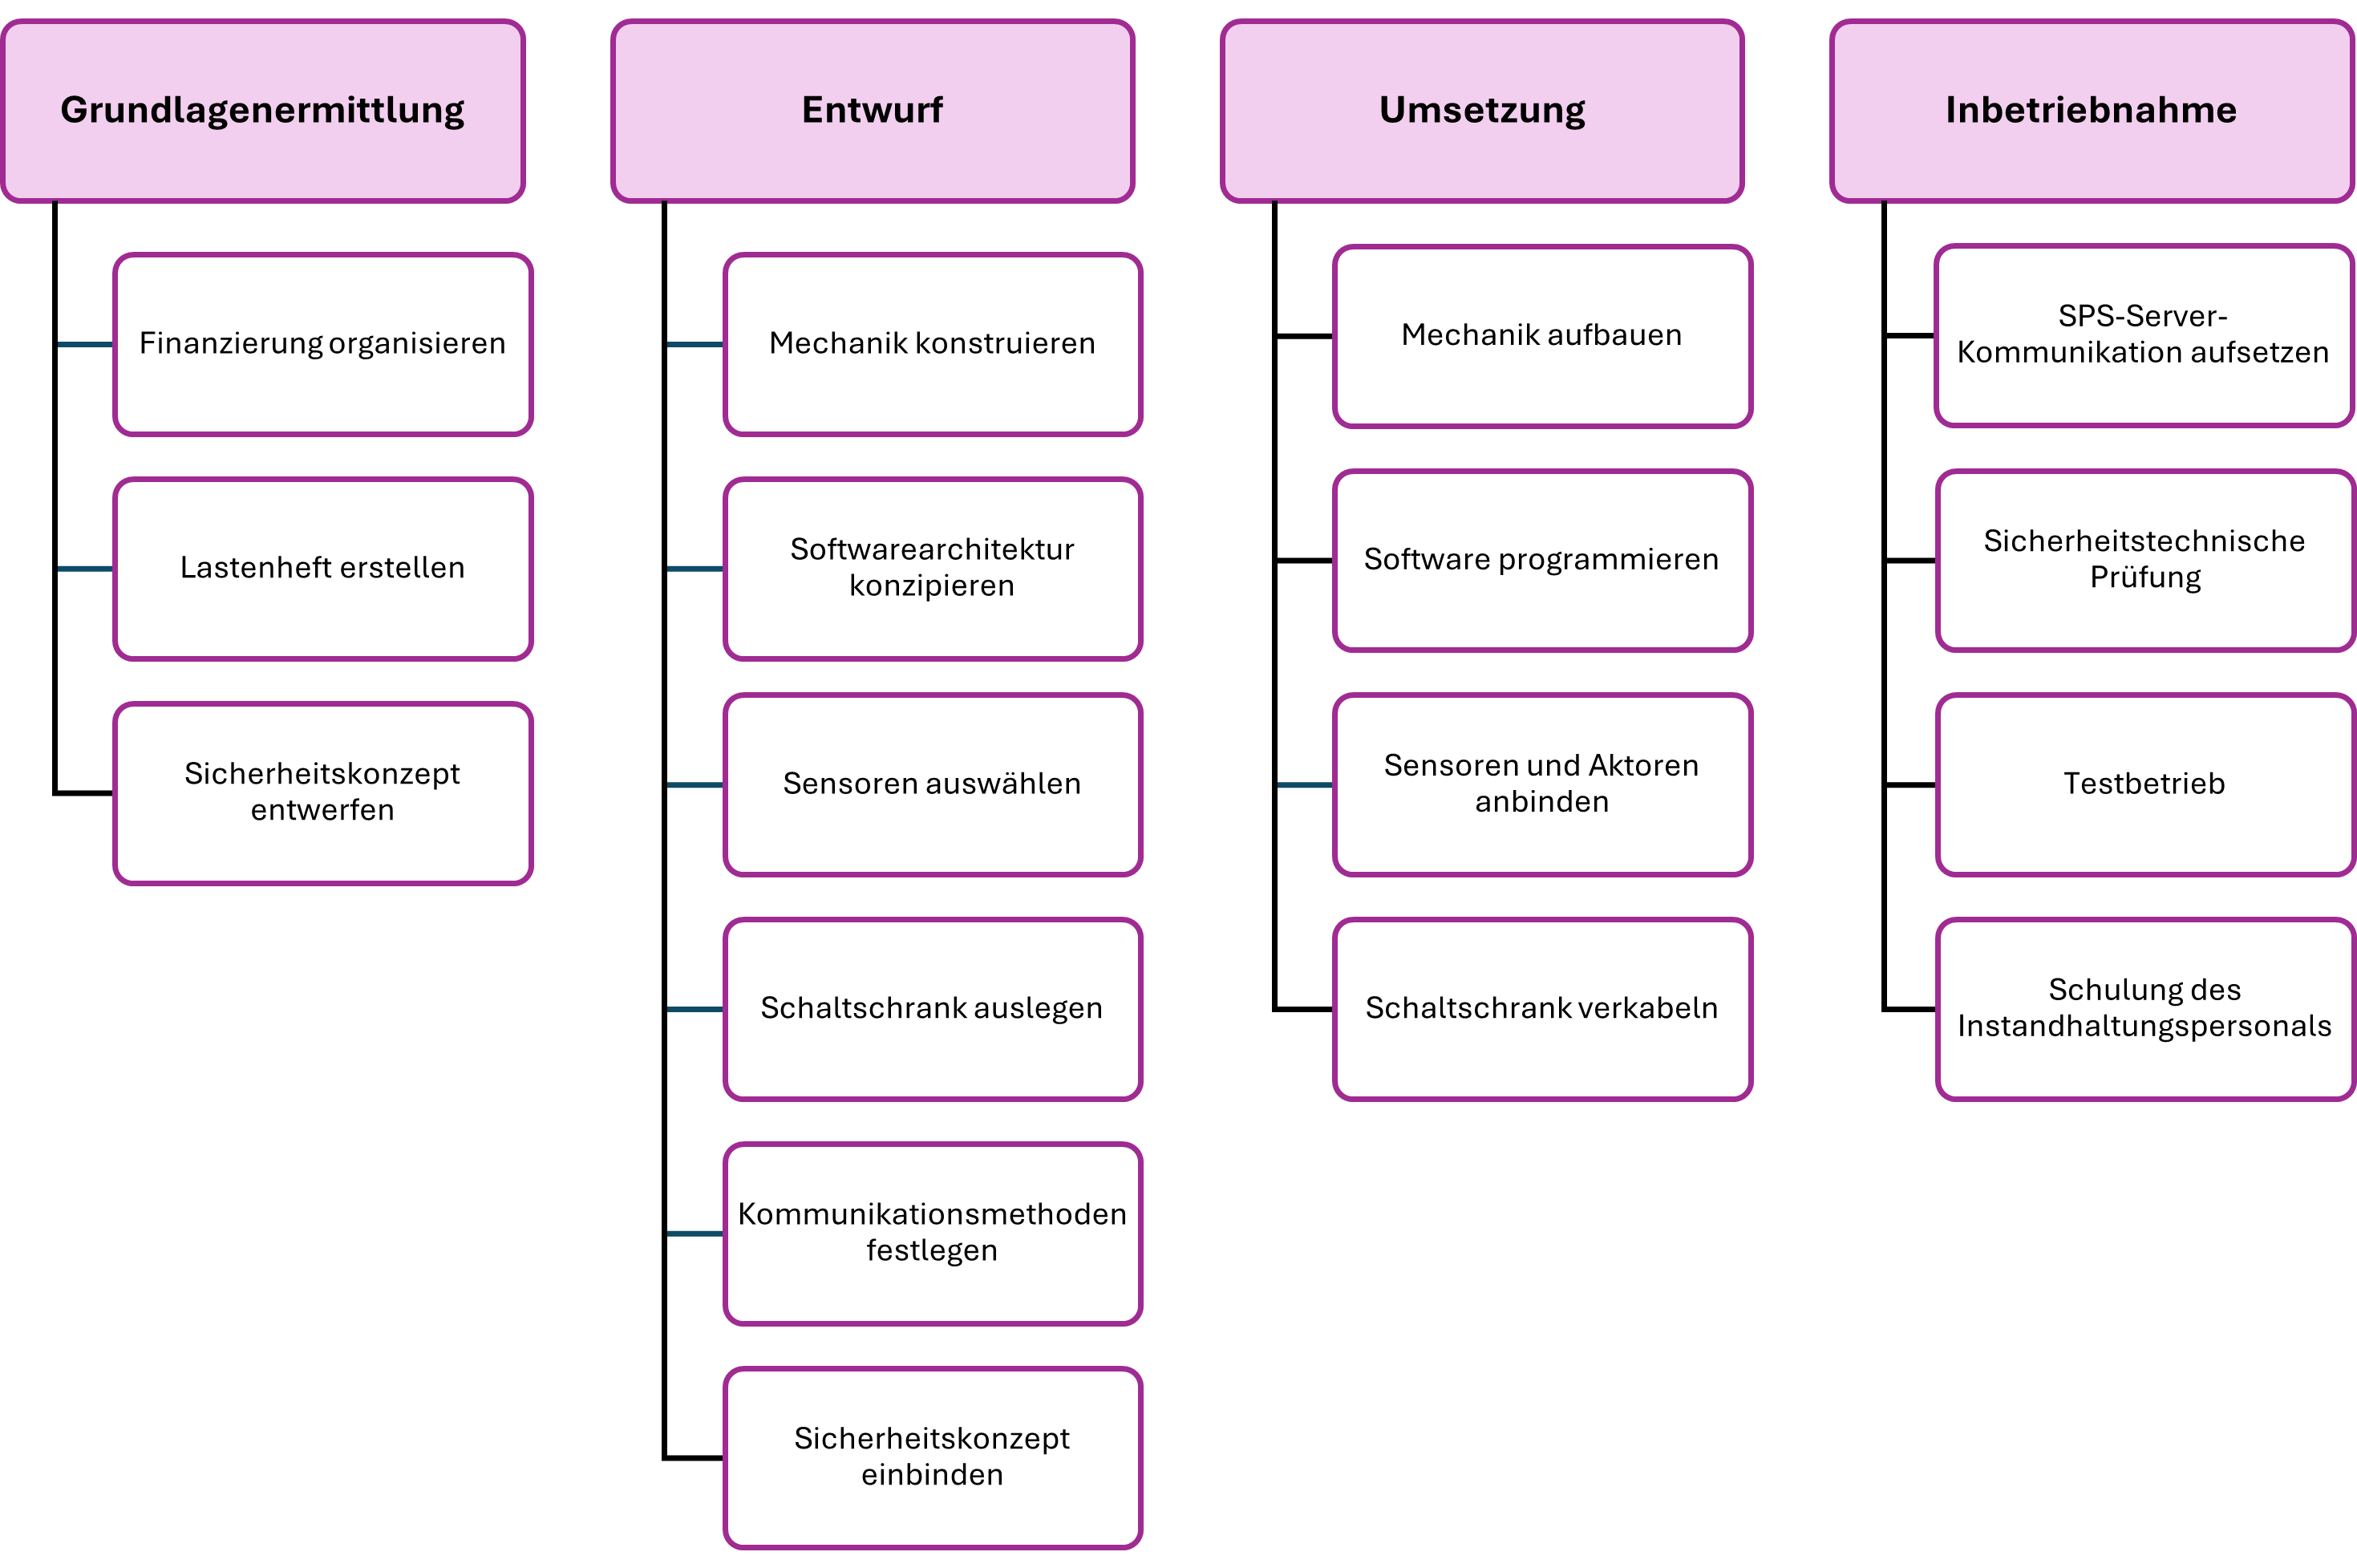
\includegraphics[width=0.9\textwidth]{ProjektStrukturPlan.png}
    \captionof{figure}{Projektstrukturplan}
\egroup

\newpage
\subsubsection{Terminplanung}
\vspace{5mm}

\bgroup
    \centering
    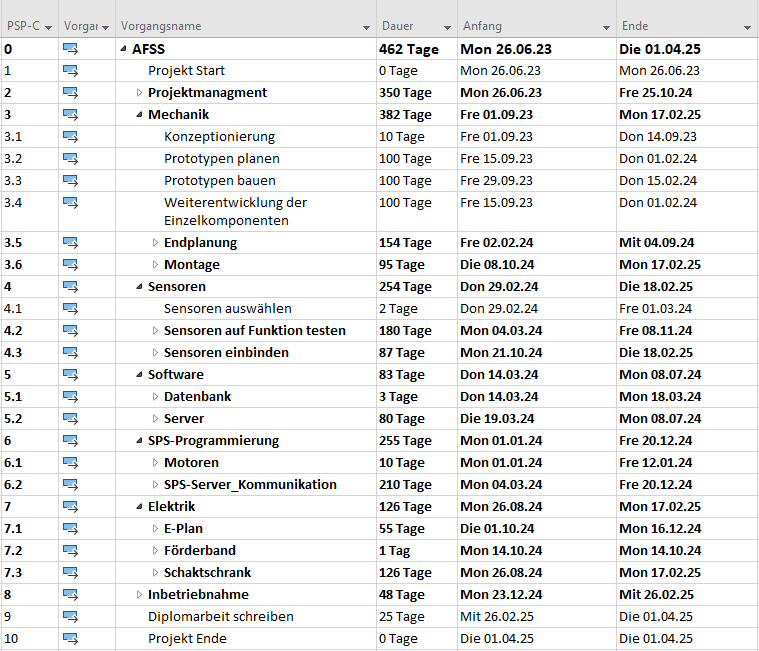
\includegraphics[width=1\textwidth]{Terminplanung.png}
    \captionof{figure}{Terminplanung in MS Project}
\egroup

\newpage

\subsubsection{Arbeitspakete}

\paragraph{Maschinenbau (Simbürger)}
\begin{itemize}
    \item Konzeptionierung des Gesamtsystem
    \item CAD - Planung
    \item Komponentenfertigung
    \item Aufbau 
\end{itemize}

\paragraph{Softwareentwicklung (Simbürger)}
\begin{itemize}
    \item Benutzeroberfläche
    \item Warehouse Management System
    \item Datenbanken
\end{itemize}

\paragraph{Elektrische Planung und Realisierung (Voglauer)}
\begin{itemize}
    \item Dokumentation vorhandener Geräte und Abmessungen dieser sowie vom Serverschrank 
    \item Zeichnen des Serverschrankes in Fusion 360
    \item Zeichnen der Module in Fusion 360
    \item Zeichnen des Schaltplanes in E-Plan 
    \item Zeichnen von Topologien und Übersichten in E-Plan 
    \item Herstellung von Modulen 
    \item Umbauten am Serverschrank
    \item Verdrahtung des Schaltschrankes
\end{itemize}

\paragraph{Sensorik (Widmann)}
\begin{itemize}
    \item Auswahl der Sensoren
    \item Referenzplatine
    \item Funktionsprüfungen und Messungen
    \item AS-Interface
\end{itemize}

\paragraph{Sicherheitstechnik (Widmann)}
\begin{itemize}
    \item Entwicklung eines Sicherheitskonzepts
    \item Realisierung
\end{itemize}




\newpage

\subsection{Inbetriebnahme}

\subsubsection{Server}

Der Server kann auf zwei unterschiedliche Arten in Betrieb genommen werden.  

\paragraph{Entwicklungsmodus} \mbox{}\\ 

Um beim Entwickeln einen angenehmeren Prozessablauf zu ermöglichen, kann der Server klassisch durch Starten des Programms mit Python ausgeführt werden.  
Hierzu sollte zuerst eine neue virtuelle Python-Umgebung aufgesetzt und die Pakete aus der Datei \texttt{requirements.txt} geladen werden. Alternativ kann die beim Entwickeln verwendete virtuelle Umgebung im \texttt{.conda}-Ordner genutzt werden.  

Nach Aktivierung der virtuellen Umgebung kann der Server durch Ausführen des Befehls  
\begin{verbatim}
python __init__.py
\end{verbatim}  
im Ordner \texttt{Prototyp\_2} gestartet werden.  
Im Terminal erscheinen dann die Logs des Einschaltvorgangs, einschließlich der IP-Adresse und des Ports, auf dem der Server läuft.  
Jedoch muss die Datenbank, um eine Verbindung herstellen zu können, separat gestartet werden.  
Die Verbindungsdaten für die Datenbank sowie viele weitere Konfigurationen können in der Datei \texttt{config.py} angepasst werden.  

\paragraph{Docker} \mbox{}\\

Für einen Serverbetrieb in einer Produktionsumgebung besteht die Möglichkeit, den Server über einen Docker-Container zu starten.  
Nach der Installation von Docker muss im übergeordneten Ordner von \texttt{Prototyp\_2}, in dem sich die Datei \texttt{docker-compose.yml} befindet, folgender Befehl ausgeführt werden:  

\begin{verbatim}
docker compose -f 'docker-compose.yml' up -d --build
\end{verbatim}  

Dadurch wird ein Container erstellt, der anschließend entweder in Docker-Desktop oder über die Kommandozeile gestartet werden kann.  
Da die Datenbank beim ersten Start auf einer Fremdmaschine noch kein Setup durchlaufen hat, ist es ratsam, sie mit einer Sicherungsdatei aus dem Ordner \texttt{DB\_export} aufzusetzen.  
Danach bleiben die Daten auch nach dem Abschalten des Containers erhalten.  

Jedoch ist es nach der Implementierung des Rust-Pakets noch nicht möglich, die benötigten Bibliotheken zu installieren, da diese nicht im \texttt{docker-compose.yml} enthalten sind. 



\subsubsection{Schaltschrank}
    Der Schaltschrank ist möglichst benutzerfreundlich. Zum Inbetriebnehmen ist eine Starkstromleitung an den dafür vorgesehenen Klemmen zu legen. Ist dies gegeben muss der Dreh-Trennschalter nun geschalten werden und die Anlage wird versorgt. Um die Anlage freizugeben ist der Schlüsselschalter zu betätigen.\\
    Beim Inbetriebnehmen ist zu beachten, dass keine Warnleuchten an den elektirschen Komponenten leuchten und es ist auf untypische Geräusche oder Gerüche zu achten. Bei etwaigen Auffälligkeiten ist die Anlage sofort mitels Trennschalter freizuschalten und daraufhin soll die Quelle der Auffälligkeit gefunden werden und, wenn vorhanden, der Fehler behoben werden.\\
    Zur Inbetriebnahme gehört auch, dass der FI und der Leitungsschutzschalter einmal getestet beziehungsweise geschalten werden um die Funktion zu testen.\\
\newpage
\subsection{Kostenaufstellung BSNV}
\textcolor{blue}{Für die Kalkulation im Gesamtprojekt sind folgende Kosten zu erfassen: \\
•	Kosten für Material (Hard- und Software)\\
•	externe Kosten (z.B.: Zukauf von Sensoren, Funkmodule, spezielle Entwicklungsum-gebungen, etc.) 
}
\begin{figure}[h]
    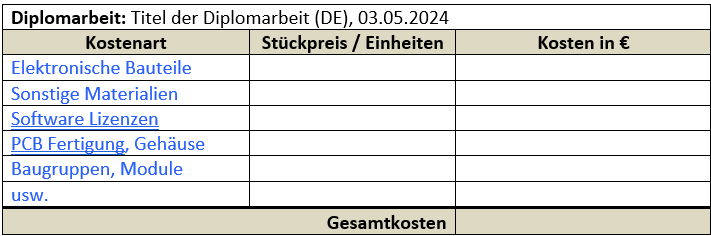
\includegraphics[width=0.8\textwidth]{Kostenaufstellung.png}
    \centering
    \caption{Kostenaufstellung}
\end{figure}


\newpage
\subsubsection{Elektrische Komponenten (Voglauer)}
Da die Käufe der Komponenten, von der Schule oder von den Sponsoren, überwiegend vor langer Zeit getätigt. Daher sind spezifische Kaufdaten nicht bekannt, die folgenden Daten schätzen somit den aktuellen Preis der Komponenten ab.\\ 
\paragraph{Kapital von der Schule}
\begin{longtable}{|p{7cm}|r|r|}
    \hline
    \textbf{Komponente} & \textbf{Stückzahl} & \textbf{Preis} \\
    \hline
    \endfirsthead

    \hline
    \textbf{Komponente} & \textbf{Stückzahl} & \textbf{Preis} \\
    \hline
    \endhead

    \hline
    \endfoot

    \hline
    \endlastfoot
    Trennschalter & 1 & € 143,00 \\
    Schlüsselschalter & 1 & € 4,99 \\
    Not-Aus-Schalter & 4 & € 12,65 \\
    Motorschutzschalter & 1 & € 55,45 \\
    Fehlerstromschutzschalter Typ A & 1 & € 221,20 \\
    Leitungsschutzschalter C13 & 1 & € 25,00 \\
    3RK2200-0CE02-0AA2 & 7 & € 146,01 \\
    6ES7155-6AU01-0CN0 & 1 & € 300,00 \\
    6ES7193-6AR00-0AA0 & 1 & € 106,67 \\
    3RK7137-6SA00-0BC1 & 1 & € 673,04 \\
    6ES7193-6BP20-0DC0 & 1 & € 70,00 \\
    Asynchronmotor & 1 & € 200,00 \\
    CL57T(V4.0) & 4 & € 36,39 \\
    TB6560 & 3 & € 17,99 \\
    23E1K-20 & 4 & € 38,77 \\
    17HS4417P1-X4 & 3 & € 8,99 \\
    \textbf{Summe} & & € 3251,00\\
    \hline
    \hline
\end{longtable}
\paragraph{Gesponsort von der KNAPP AG}
\begin{longtable}{|p{7cm}|r|r|}
    \hline
    \textbf{Komponente} & \textbf{Stückzahl} & \textbf{Preis} \\
    \hline
    \endfirsthead

    \hline
    \textbf{Komponente} & \textbf{Stückzahl} & \textbf{Preis} \\
    \hline
    \endhead

    \hline
    \endfoot

    \hline
    \endlastfoot
    \hline
    \hline
    TSX-SUP-A054 & 1 & € 250,00 \\
    6EP1436-3BA00-8AA0 & 1 & € 350,00 \\
    DP500IP/3-24 & 1 & € 301,68 \\
    DRT-240-24 & 1 & € 97,46 \\
    6ES7515-2AN03-0AB0 & 1 & € 3.195,40 \\
    6ES7521-1BL00-0AB0 & 1 & € 332,10 \\
    6ES7553-1AA00-0AB0 & 2 & € 825,86 \\
    6ES7522-1BL01-0AB0 & 1 & € 560,49 \\
    \textbf{Summe} & & € 5.912,99\\
\end{longtable}
\paragraph{Gesponsort von der Weidmüller GmbH}
\begin{longtable}{|p{7cm}|r|r|}
    \hline
    \textbf{Komponente} & \textbf{Stückzahl} & \textbf{Preis} \\
    \hline
    \endfirsthead

    \hline
    \textbf{Komponente} & \textbf{Stückzahl} & \textbf{Preis} \\
    \hline
    \endhead

    \hline
    \endfoot

    \hline
    \endlastfoot
    \hline
    \hline
    2081870000 & 2 & € 8,41 \\
    IE-FC-SET-SPDEK001-KY-P & 1 & € 144,93 \\
    2080600000 & 4 & € 37,26 \\
    2080480000 & 2 & € 37,18 \\
    AL2C 2.5 & 100 & € 0,64 \\
    \textbf{Summe} & & € 449,15\\
\end{longtable}
\paragraph{Gesponsort von der Firma Lapp}
\begin{longtable}{|p{7cm}|r|r|}
    \hline
    \textbf{Komponente} & \textbf{Stückzahl} & \textbf{Preis} \\
    \hline
    \endfirsthead

    \hline
    \textbf{Komponente} & \textbf{Stückzahl} & \textbf{Preis} \\
    \hline
    \endhead

    \hline
    \endfoot

    \hline
    \endlastfoot
    \hline
    \hline
    ÖLFLEX CLASSIC FD 810 CY 5x0.5 & 30m & € 117,63 \\
    ÖLFLEX CLASSIC FD 810 CY 5x0.75 & 40m & € 174,41 \\
    ÖLFLEX CHAIN 809 CY 7x0.5 & 40m & € 150,95 \\
    H05V-K 1x0.75 & 100m & € 18,86 \\
    H05V-K 1x0.75 & 100m & € 18,86 \\
    H05V-K 1x0.75 & 100m & € 18,86 \\
    \textbf{Summe} & & € 496,57\\
\end{longtable}

\subsection{Kostenaufstellung des AFSS}
Da die Käufe der Komponenten, von der Schule oder von den Sponsoren, überwiegend vor langer Zeit getätigt. Daher sind spezifische Kaufdaten nicht bekannt, die folgenden Daten schätzen somit den aktuellen Preis der Komponenten ab. 
\paragraph{Kapital von der Schule}\mbox{}\\
\begin{table}[H]
    \begin{tabular}{lllll}
    Name                & Artikelnummer                          & Menge & pro Stück {[}€{]} & Preis {[}€{]} \\ \hline
    Trennschalter       & -                                     & 1     & 143.00            & 143.00        \\
    Schlüsselschalter   & -                                     & 1     & 4.99              & 4.99          \\
    Not-Aus-Schalter    & -                                     & 4     & 12.65             & 50.60         \\
    Motorschutzschalter & -                                     & 1     & 55.45             & 55.45         \\
    Fehlerstromschutzschalter Typ A & -                         & 1     & 221.20            & 221.20        \\
    Leitungsschutzschalter C13 & -                             & 1     & 25.00             & 25.00         \\
    ASi-Slaves          & 3RK2200-0CE02-0AA2                   & 7     & 146.01            & 1022.07       \\
    ET 200 SP           & 6ES7155-6AU01-0CN0                   & 1     & 300.00            & 300.00        \\
    Bus-Karte           & 6ES7193-6AR00-0AA0                   & 1     & 106.67            & 106.67        \\
    ASi-Master-Karte    & 3RK7137-6SA00-0BC1                   & 1     & 673.04            & 673.04        \\
    ASi-Steckadapter    & 6ES7193-6BP20-0DC0                   & 1     & 70.00             & 70.00         \\
    Asynchronmotor      & -                                     & 1     & 200.00            & 200.00        \\
    SM-Treiber          & CL57T(V4.0)                          & 4     & 36.39             & 145.56        \\
    SM-Treiber          & TB6560                               & 3     & 17.99             & 53.97         \\
    Schrittmotor        & 23E1K-20                             & 4     & 38.77             & 155.08        \\
    Schrittmotor        & 17HS4417P1-X4                        & 3     & 8.99              & 26.97         \\ \hline
    Gesamt              &                                      &       &                   & 3251.00       
    \end{tabular}
\end{table}
\paragraph{Gesponsort von der KNAPP AG}\mbox{}\\
\begin{table}[H]
    \begin{tabular}{lllll}
    Name                & Artikelnummer                          & Menge & pro Stück {[}€{]} & Preis {[}€{]} \\ \hline
    ASi-Netzteil        & TSX-SUP-A054                           & 1     & 250.00            & 250.00        \\
    Netzteil            & 6EP1436-3BA00-8AA0                    & 1     & 350.00            & 350.00        \\
    Netzteil            & DP500IP/3-24                          & 1     & 301.68            & 301.68        \\
    Netzteil            & DRT-240-24                            & 1     & 97.46             & 97.46         \\
    SPS                 & 6ES7515-2AN03-0AB0                    & 1     & 3195.40           & 3195.40       \\
    SPS-DI-Karte        & 6ES7521-1BL00-0AB0                    & 1     & 332.10            & 332.10        \\
    SPS-PTO-Karte       & 6ES7553-1AA00-0AB0                    & 2     & 825.86            & 1651.72       \\
    SPS-DO-Karte        & 6ES7522-1BL01-0AB0                    & 1     & 560.49            & 560.49        \\ \hline
    Gesamt              &                                        &       &                   & 5912.99       
    \end{tabular}
\end{table}
\paragraph{Gesponsort von der Weidmüller GmbH}\mbox{}\\
\begin{table}[H]
    \begin{tabular}{lllll}
    Name                & Artikelnummer                          & Menge & pro Stück {[}€{]} & Preis {[}€{]} \\ \hline
    Feed-In-Module      & 2081870000                             & 2     & 8.41              & 16.82         \\
    Service-Schnittstelle & IE-FC-SET-SPDEK001-KY-P               & 1     & 144.93            & 144.93        \\
    8A DC Sicherung     & 2080600000                             & 4     & 37.26             & 149.04        \\
    2A DC Sicherung     & 2080480000                             & 2     & 37.18             & 74.36         \\
    Reihenklemme        & AL2C 2.5                               & 100   & 0.64              & 64.00         \\ \hline
    Gesamt              &                                        &       &                   & 449.15       
    \end{tabular}
\end{table}
\paragraph{Gesponsort von der Firma Lapp}\mbox{}\\
\begin{table}[H]
    \begin{tabular}{lllll}
    Name                & Artikelnummer                          & Menge & pro Stück {[}€{]} & Preis {[}€{]} \\ \hline
    Kabel               & ÖLFLEX CLASSIC FD 810 CY 5x0.5         & 30m   & 3.92              & 117.63        \\
    Kabel               & ÖLFLEX CLASSIC FD 810 CY 5x0.75        & 40m   & 4.36              & 174.41        \\
    Kabel               & ÖLFLEX CHAIN 809 CY 7x0.5              & 40m   & 3.77              & 150.95        \\
    Verdrahtungsdraht   & H05V-K 1x0.75                          & 100m  & 0.19              & 18.86         \\
    Verdrahtungsdraht   & H05V-K 1x0.75                          & 100m  & 0.19              & 18.86         \\
    Verdrahtungsdraht   & H05V-K 1x0.75                          & 100m  & 0.19              & 18.86         \\ \hline
    Gesamt              &                                        &       &                   & 496.57       
    \end{tabular}
\end{table}
\paragraph{Gesamtwert der elektrischen Komponenten}\mbox{}\\
    Alle bisher gelisteten Komponenten gemeinsam verfügen über einen Geschätzten Wert von 10 109,71 €.\\ 
    Zuzüglich des Serverschrankes und den Materialkosten der Montageplatten beträgt der gesammte Schätzwert für den Schaltschrank zwischen 12 000 und 14,500€.
\paragraph{Gesponsort von der Igus GmbH}\mbox{}\\
\begin{table}[H]
    \begin{tabular}{llllll}
    Name                & Artikelnummer          & Menge & pro Stück {[}€{]} & Preis {[}€{]} \\ \hline
    Schlepkette X       & E2i.26.057.048.0       & 1             & 72.72                   & 72.72         \\
    Schlepkette Y       & E2i.26.038.048.0       & 1             & 49.74                   & 49.74         \\
    Gewindespindel      & DST-LS-10X12-R-ES      & 2 x 350mm              & 35.15                   & 70.3          \\
    Gewindemutter       & DST-JFRM-252525DS10X12 & 2             & 26.33                   & 52.66         \\
    Führungsschiene     & TS-01-20               & 2 x 350mm              & 16.685                  & 33.37         \\
    Führungswagen       & TW-01-20               & 2             & 35.1                    & 70.2          \\ \hline
    Gesamt              &                        &               &                         & 348.99       
    \end{tabular}
\end{table}

\paragraph{Gesponsort von der Mädler GmbH}\mbox{}\\
\begin{table}[H]
    \begin{tabular}{lllll}
    Name                           & Artikelnummer & Menge & pro Stück {[}€{]} & Preis {[}€{]}  \\ \hline
    Zahnscheibe AT5x16 20 Zähne    & 16632000      & 2     & 7.58            & 15.16  \\
    Zahnscheibe AT5x16    27 Zähne & 16632700      & 2     & 8.7             & 17.4   \\
    Zahnscheibe AT5x16  36 Zähne   & 16633600      & 2     & 12.58           & 25.16  \\
    Zahnriemen AT5x16              & 16670000      & 21    & 16.44           & 345.24 \\ \hline
    Gesamt                         &               &       &                 & 402.96
    \end{tabular}
\end{table}
\newpage
\subsection{Besprechungsprotokolle (SV)}
%include pdf file as image, on howl page with label
\begin{figure}[H]
    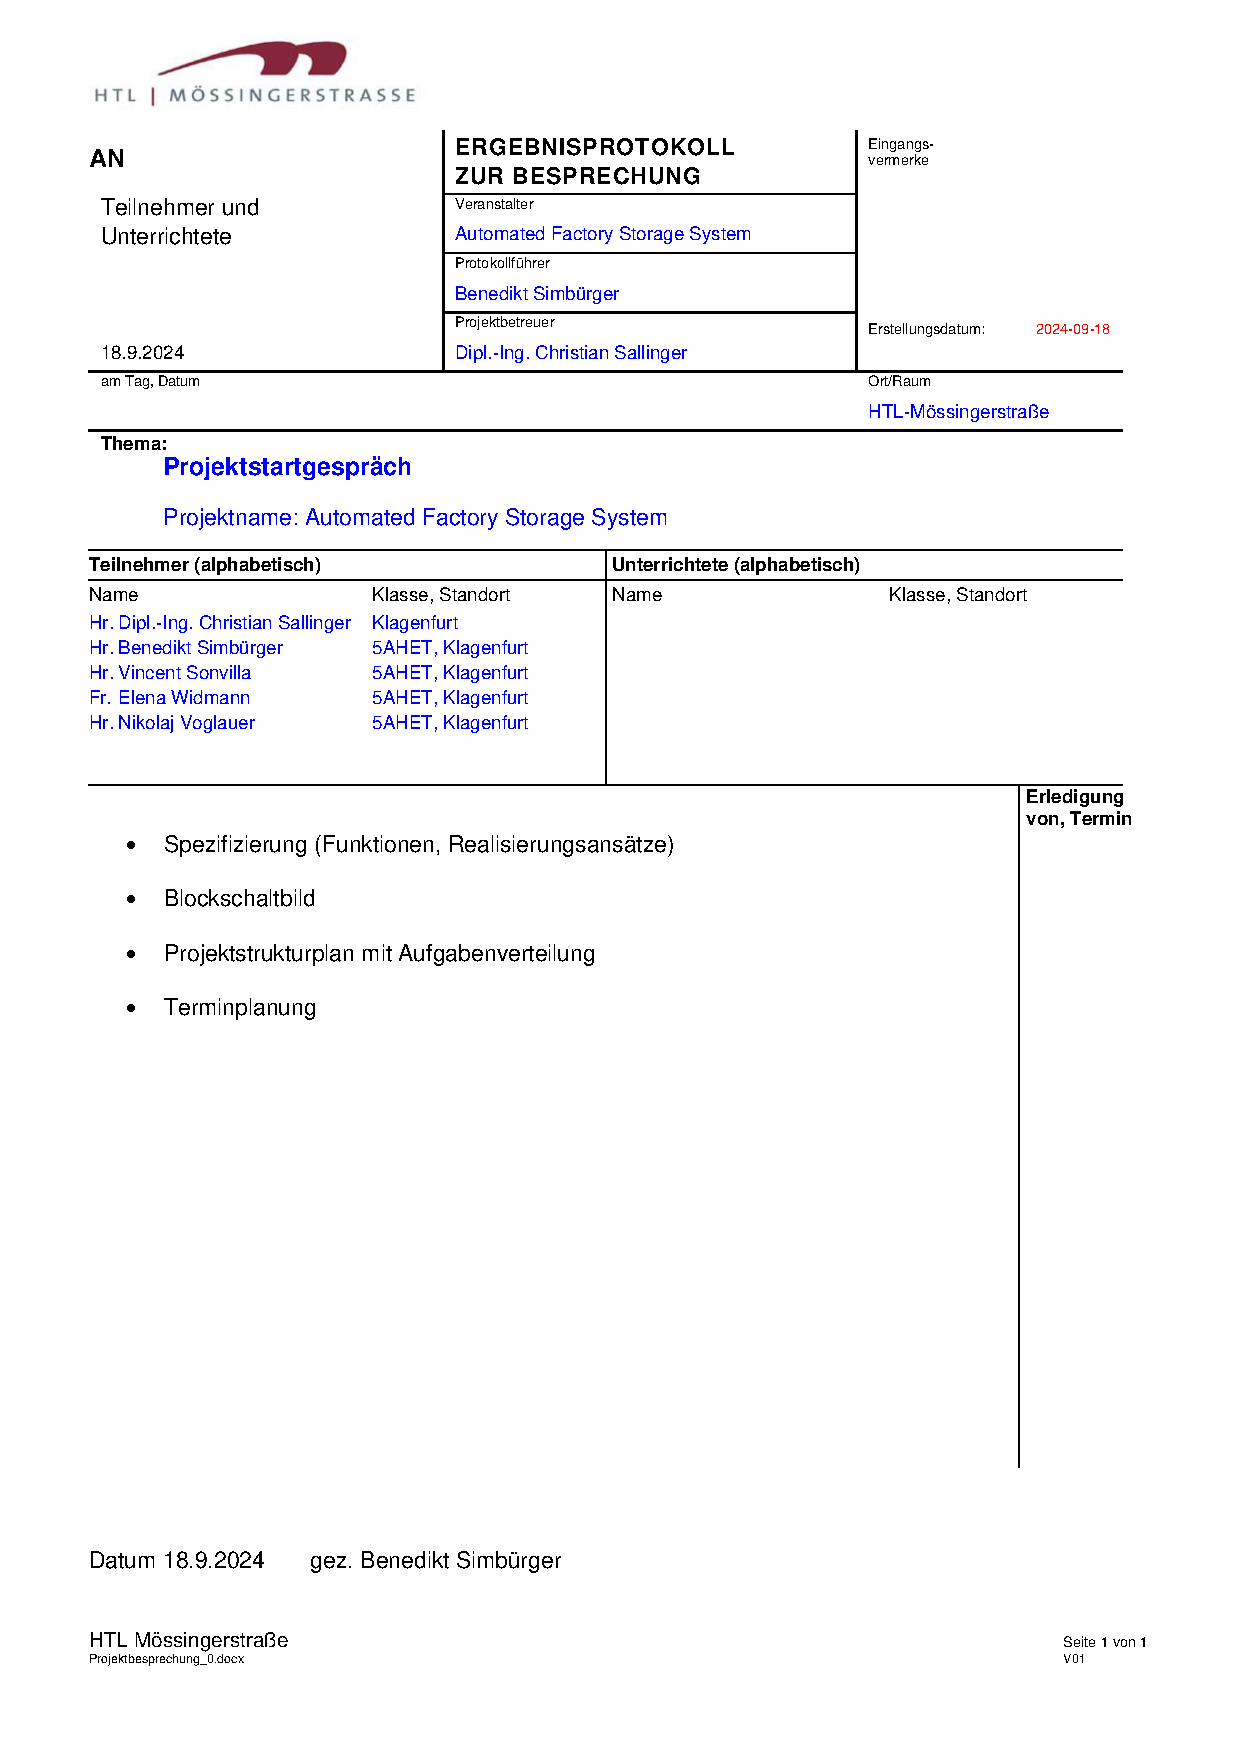
\includegraphics[width=0.9\textwidth]{../Protokolls/Projektbesprechung_0.pdf}
    \centering
    \caption{Besprechungsprotokoll 10.12.2024}
\end{figure}

\begin{figure}[H]
    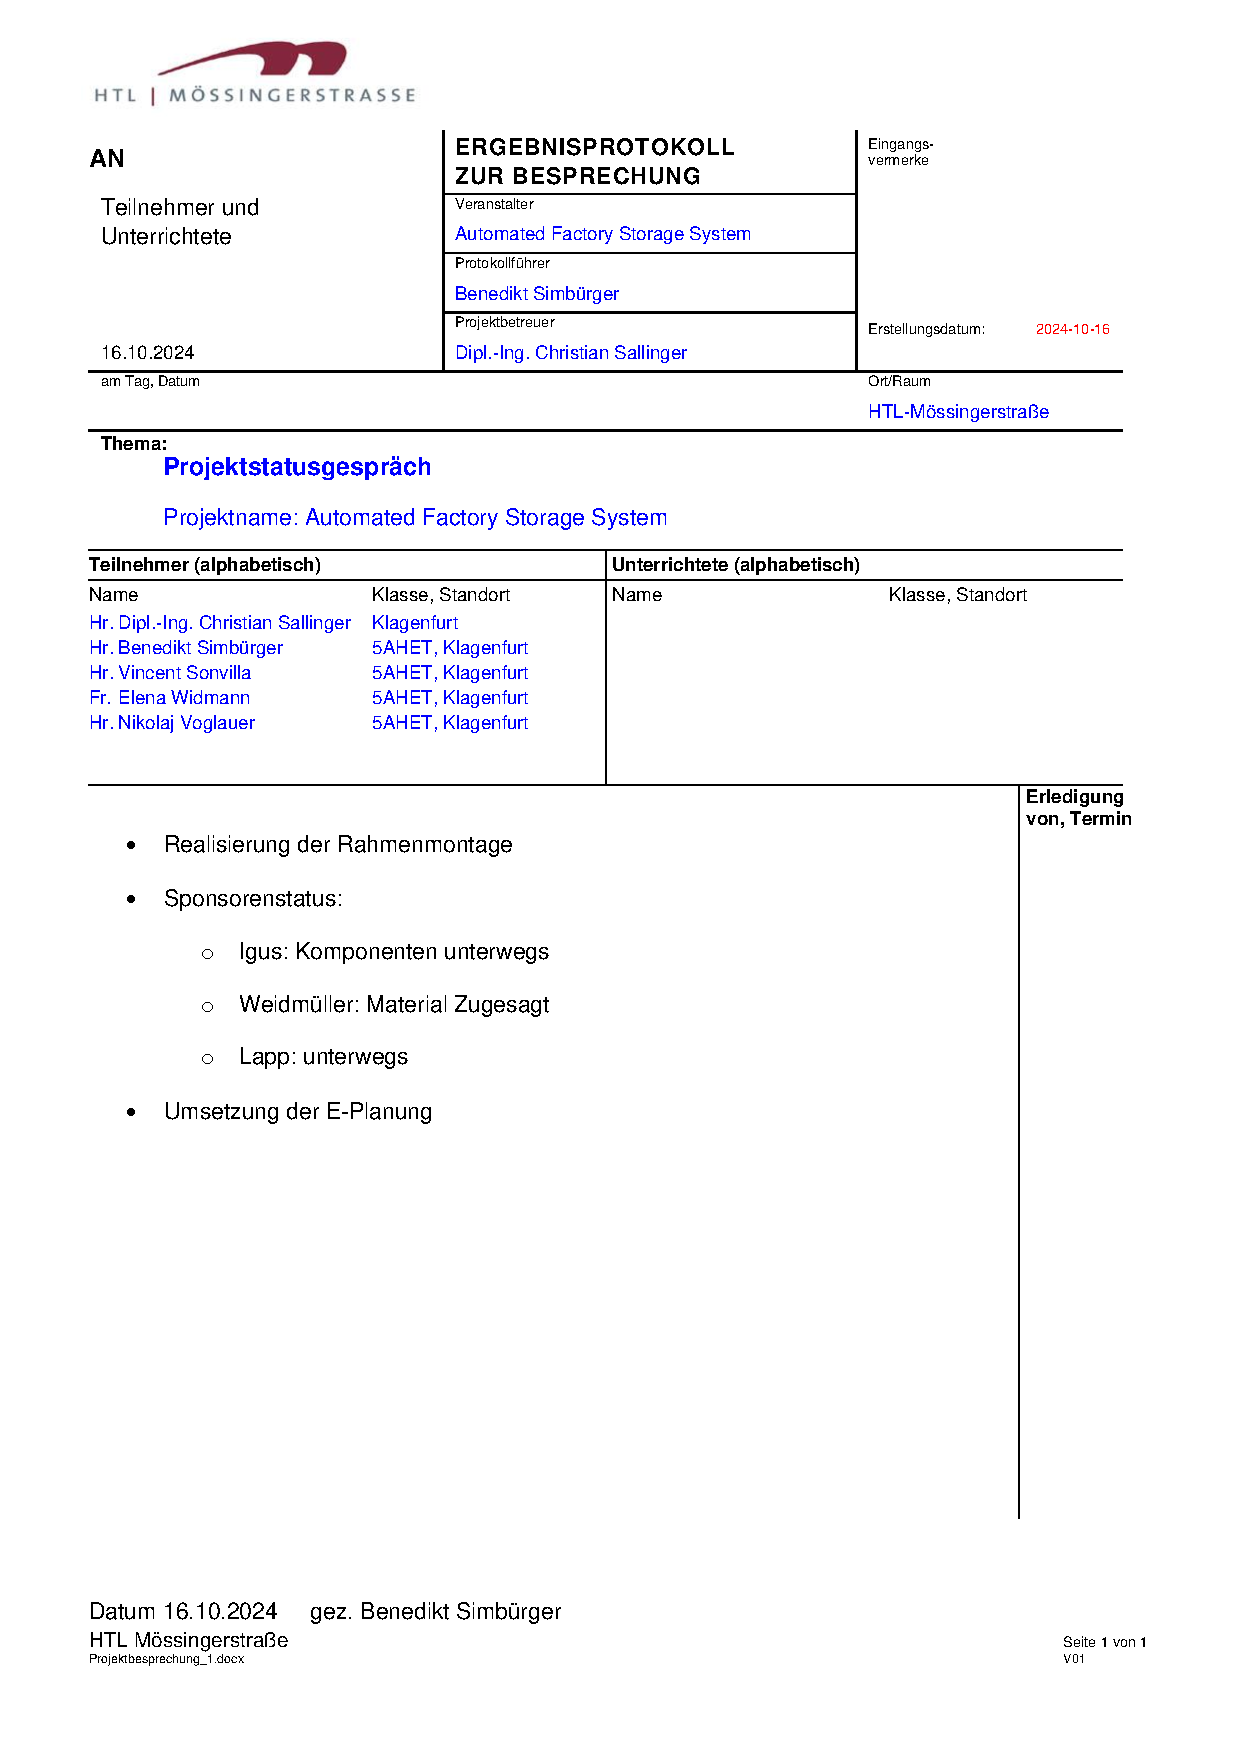
\includegraphics[width=0.9\textwidth]{../Protokolls/Projektbesprechung_1.pdf}
    \centering
    \caption{Besprechungsprotokoll 16.10.2024}
\end{figure}

\begin{figure}[H]
    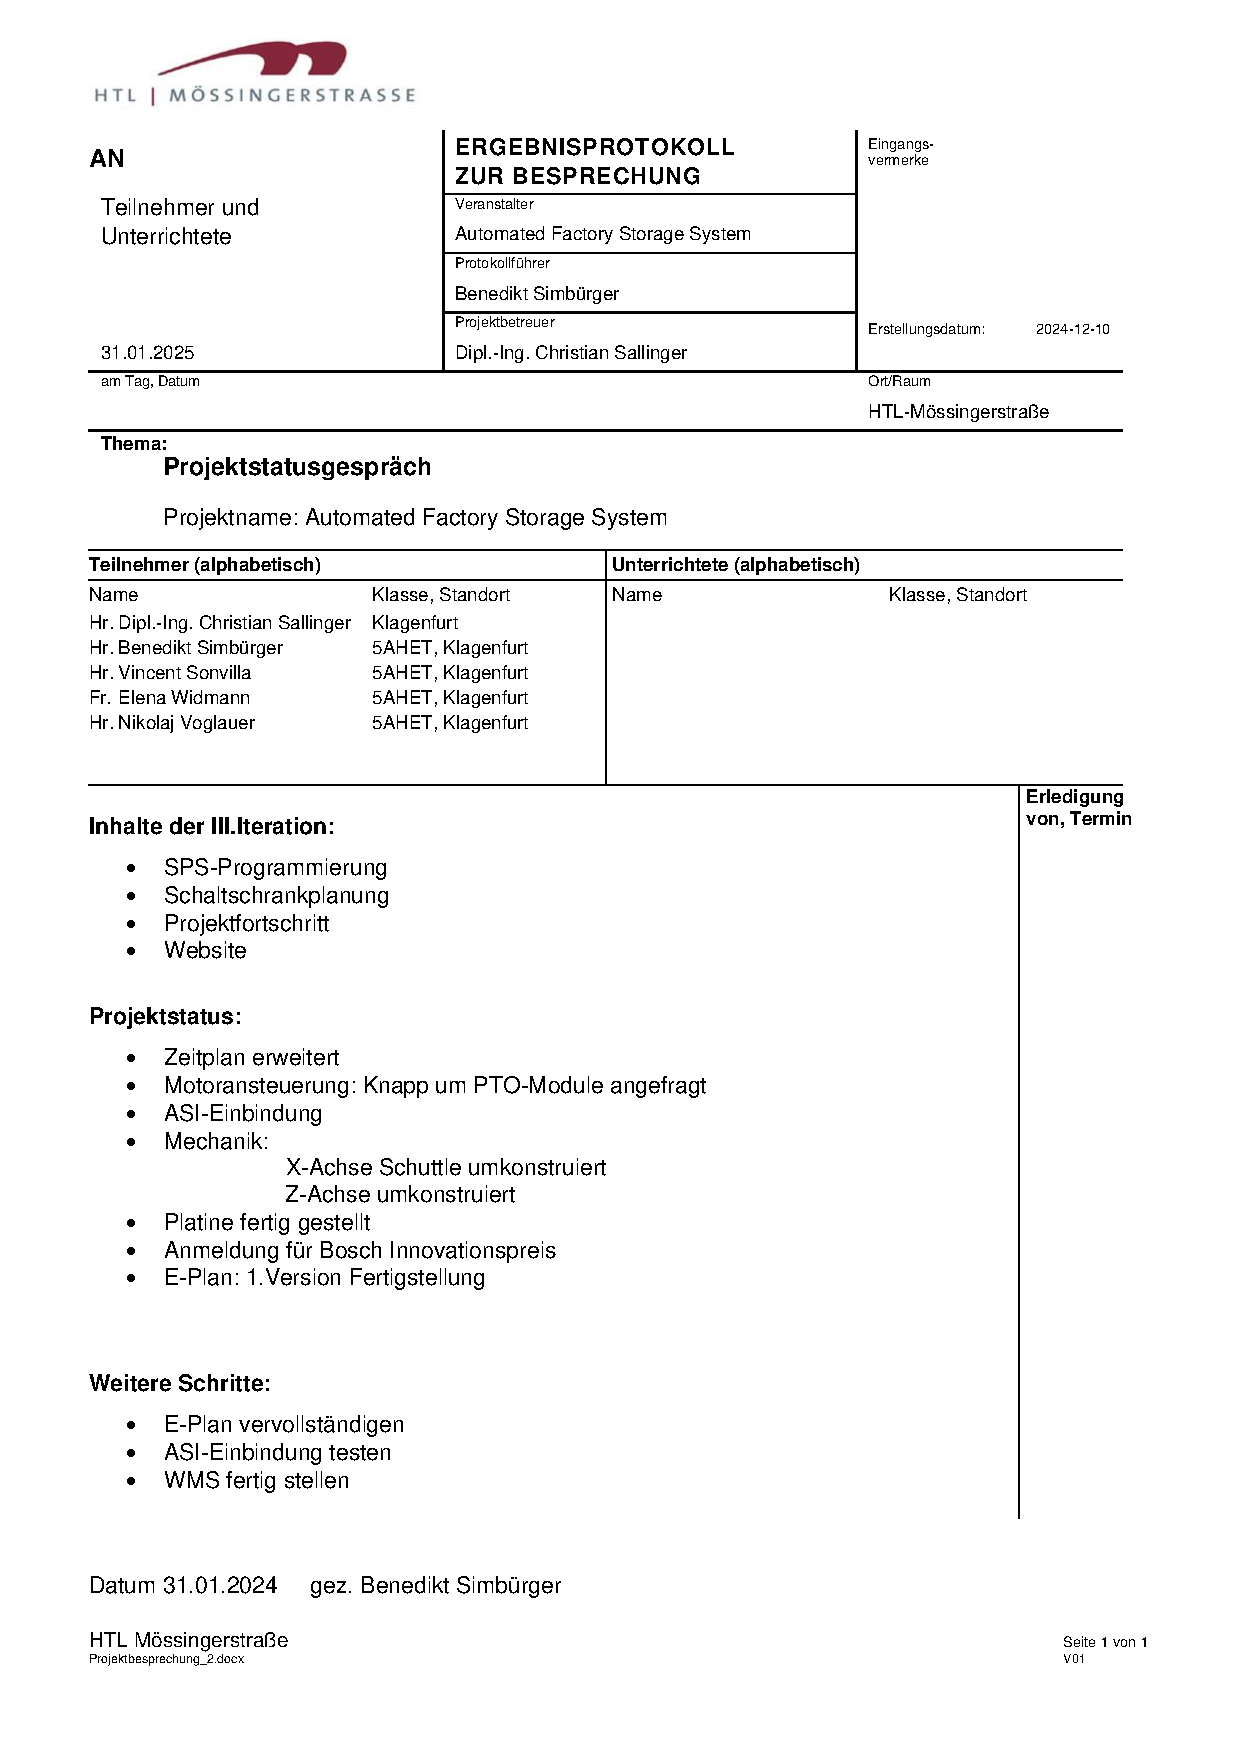
\includegraphics[width=0.9\textwidth]{../Protokolls/Projektbesprechung_2.pdf}
    \centering
    \caption{Besprechungsprotokoll 10.12.2024}
\end{figure}

\begin{figure}[H]
    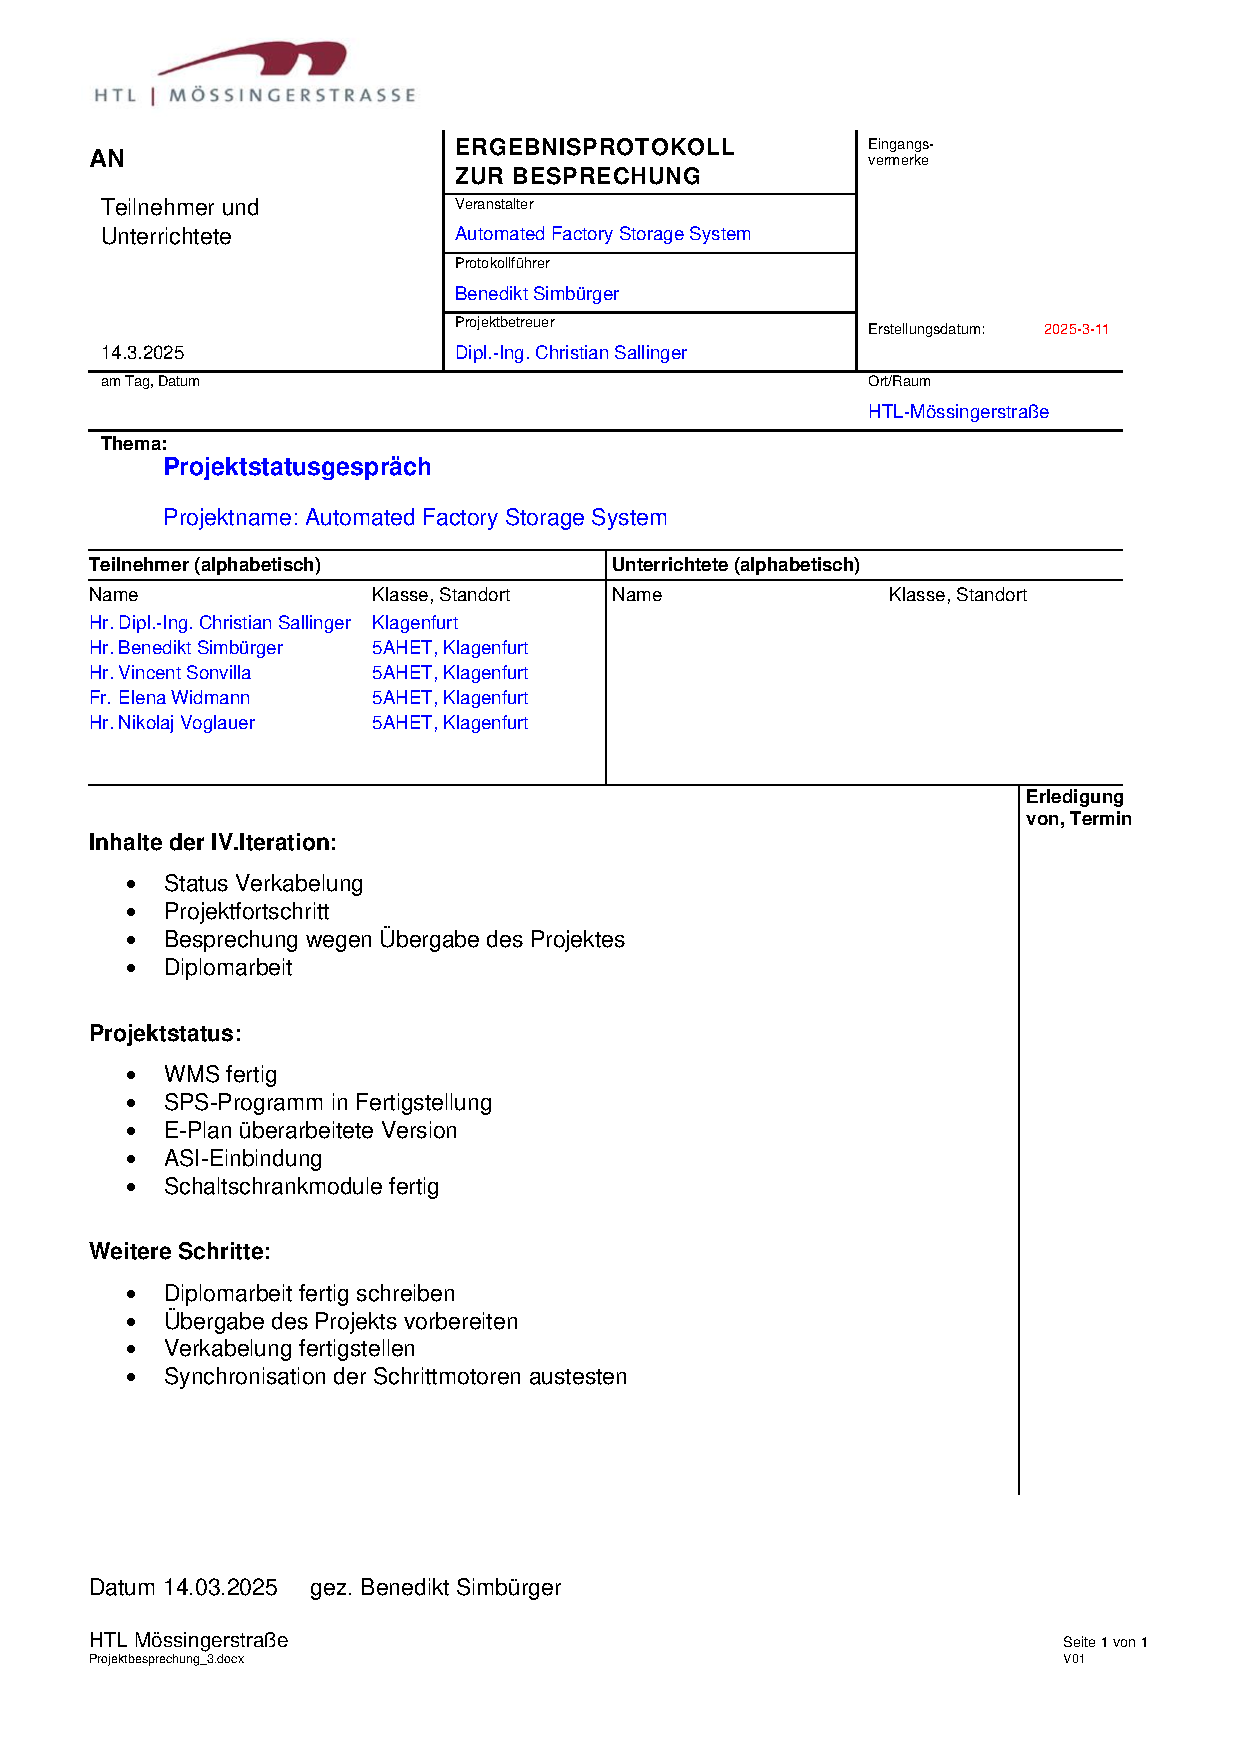
\includegraphics[width=0.9\textwidth]{../Protokolls/Projektbesprechung_3.pdf}
    \centering
    \caption{Besprechungsprotokoll x.x.xxxx}
\end{figure}




\newpage
\subsection{Arbeitsnachweis}

\subsubsection{Simbürger}

\begin{longtable}{|l|p{10cm}|r|}
    \hline
    \textbf{Datum} & \textbf{Tätigkeit} & \textbf{Stunden} \\
    \hline
    \endfirsthead

    \hline
    \textbf{Datum} & \textbf{Tätigkeit} & \textbf{Stunden} \\
    \hline
    \endhead

    \hline
    \endfoot

    \hline
    \endlastfoot

4.10.2023&Besprechung des weiteren vorgehens mit WB	&0.5\\
9.10.2023&Gruppenbesprechung für das weitere Vorgehen	&1.0\\

19.12.2023	&CAD Auf/Ab-fahrer	&3.0\\

10.1.2024	&Testversuch ET200 SPS Stepdrive und Meeting Knapp&	4.0\\
11.1.2024	&Achse mechanisch fertig, Schlitten vertikal&	4.0\\
12.1.2024	&CAD Schuttel, Tag der offenen Tür vorbereitung	&2.0\\
16.1.2024	&Motoren ansteuern&	1.0	\\
20.1.2024	&Umlenkungen- und Aufhängungskonstruktion&	4.0\\
29.1.2024	&Diagramm Datenaustausch Anfertigung&   2.0\\
1.2.2024	&Besprechung WB&	4.0\\
3.2.2024	&Website Backend/Frontend Prototyp&	9.0\\
4.2.2024	&WS Frontend&	3.0\\

5.2.2024	&KWF Antrag schreiben und WS Datenbankmanagement&	3.0\\
7.2.2024	&OPC UA Client testung&	4.5\\
15.2.2024	&WS Suche usw, Organisation, Maschinenbaubesprechung	&5.5\\

20.2.2024	&Python / OPC UA Client testen	&1.0\\
23.2.2024	&WS Warenkorb, restructuring	&9.0\\
24.2.2024	&WS Warenkorb fertig, OPC anfang und Pflichtenheft Erstversion&	6.0\\
27.2.2024	&http-Kommunikation	testen&4.0\\
28.2.2024	&Lasten/Pflichtenheft erstellen	&3.0\\
4.3.2024	&http-Kommunikation testen&	3.5\\
10.3.2024	&CAD X-Achse& 7.0\\
13.3.2024	&Absprache mit WB bez. Pflichtenheft	&1.0\\
14.3.2024	&http-Kommunikation und CAD&	3.0\\
1.4.2024	&Datenbanken und Visualisierung	&5.0\\
2.4.2024	&CAD Lagerregal&	2.0\\
17.4.2024	&CAD Gabel und Software&	2.0\\
23.4.2024	&STT-Fortsetzung / Software einführung&	2.5\\
12.4.2024	&Datenbanken und Visu	&5.0\\
21.4.2024	&Datenbanken und Visu	&5.0\\
22.4.2024	&TF-IDF Recherche	&3.0\\
23.4.2024	&TF-IDF Implementierung	&2.0\\
28.4.2024	&Areas und Locations Implementierung	&6.0\\
19.4.2024	&Order Algorithmus konzeptionieren	&3.0\\
22.5.2024	&Order Algorithmus Implementierung	&3.0\\
2.6.2024	&Order Api Programmierung	&5.0\\
3.6.2024	&Api Implementierung und Visu& 3.0\\
4.6.2024	&STT-Fortsetzung und CAD&	2.0\\
6.6.2024	&SPS/Server Communictaion und Z-Prototyp CAD	&5.0\\
8.6.2024	&SPS Comm und Simulation implement	&4.0\\
9.6.2024	&System Controller	&4.0\\

14.6.2024	&Z-Prototyp Bauteile Vorbereitung& 1.0\\
18.6.2024	&Return, Cart programmieren	&4.0\\
19.6.2024	&Docker (f me)	&3.0\\
21.6.2024	&Z-PT, Schaltschrank, SPS-Com&	4.5\\
16.7.2024	&Recherche, Referenz-Elektronik&	1.0\\
17.7.2024	&Ref-Elektronik	&2.0\\
19.7.2024	&Designe/CAD Rollen u. Spannen y &6.0\\
22.7.2024	&Design X-Spannelement	&2.0\\
25.7.2024	&Design X-Spannelement und Rollen	&1.5\\
31.7.2024	&CAD Z-Achsen zauberei &	1.0\\
1.8.2024	&CAD Z-Achse redesign & 5.0\\
9.8.2024	&CAD YZ-Achse grobe fertigstellung&	5.0\\
10.8.2024	&CAD YZ-Achse feinerschliff	&4.0\\
11.8.2024	&CAD YZ-Achse + X-Achse beginn&	2.0\\
12.8.2024	&CAD X-Achse	&1.0\\
13.8.2024	&CAD X-Achse side roller	&4.0\\
14.8.2024	&CAD X-Achse side roller 2. side	&2.0\\
15.8.2024	&CAD X-Achse Mid rollers, side Wheels, YZ-Achse Spiegelung	&6.0\\
16.8.2024	&CAD YZ-Achse Lichttaster, X-Achse	&1.0\\
17.8.2024	&X-Achse Schleppkettengedanken Auslegung	&6.0\\
19.8.2024	&Schleppenderketten einplanung	&2.0\\
20.8.2024	&CAD vertikale Schleppkette &3.0\\
20.8.2024	&Sponsoren-E-mail beginn	&1.3\\
21.8.2024	&Kontaktdaten, Projektzusammenfassung	&1.5\\
22.8.2024	&CAD Schlitten Top 	&1.0\\
24.8.2024	&Stückliste, CAD Schlitten Top	&2.0\\
25.8.2024	&CAD X-Top Verbindung, Umlenkung	&5.0\\
27.8.2024	&CAD Rahmen Aufhängungen	&2.0\\
29.8.2024	&CAD Umlenkungen und Motoraufhängungen	&5.0\\
30.8.2024	&CAD Endschalter und Rahmen beginn	&3.0\\
31.8.2024	&CAD Rahmen, Lagerschrank beginn	&6.0\\
1.9.2024	&CAD Lagerschrank und Querfördererausschnitt	&2.0\\
2.9.2024	&Verbidungsslider implementieren	&1.0\\
3.9.2024	&Bugs beheben, Weidmüller Sortiment Bauteile auswählen	&4.0\\
4.9.2024	&Stack Bug behoben und CAD Querförderer	&7.0\\
5.9.2024	&CAD Mech. weitestgehende Fertigstellung	&4.0\\
9.9.2024	&Latex aufsetzen	&2.5\\
10.9.2024	&Meeting Weidmüller&	2.0	\\
11.9.2024	&Schaltschrank konzeptionieren &2.25\\
15.9.2024	&Stückliste anfertigen	&2.0\\

17.9.2024	&Autolager Demontieren für Bauteilbeschaffung&	2.5\\
18.9.2024	&Verbindungstest, Suchalgorythmus Rust implementation &6.0\\
19.9.2024	&Suchag. Fertig implementiert, CAD Rollen gezeichnet	&3.0\\

24.9.2024	&Projektmanagement&	3.0\\
25.9.2024	&Änderungen V-Slot-Aufhängung, Project-Libre	&1.0\\

26.9.2024	&Igus, Weidmüller, Motoren ansteuern die 1.&	4.0\\
28.9.2024	&Bux im Lageralgorithmus beheben	&1.5\\

1.10.2024	&CAD	&1.0\\
3.10.2024	&Profile bearbeiten	&1.5\\
8.10.2024	&Latex Vorlage	&1.0\\
9.10.2024	&Raumeinrichtung&	3.0\\
21.10.2024	&Rahmenbau beginn&	2.0\\
22.10.2024	&Rahmenbau und Drehstromverlegung, Auftragsvorbereitung X-Aufhängung &5.5\\
23.10.2024	&Rahmenbau	&3.0\\
24.10.2024	&Rahmenbau	&3.0\\
25.10.2024	&CAD XZ-Redesign	&3.0	\\
26.10.2024	&CAD XZ-Redesign	&7.0	\\
27.10.2024	&Auftragsvorbereitung X-Achse	&3.0\\
28.10.2024	&Auftragsvorbereitung X-Achse	&2.0	\\

5.11.2024	&Beginn Umlenkrollen Drehen	&0.8\\
6.11.2024	&Weidmüller DP Inbetrtiebnahme&	1.0\\
7.11.2024	&Weidmülller DP ansteuern&	3.5\\
8.11.2024	&Weidmülller DP ansteuern&	3.5\\
12.11.2024	&Umlenkrollen Drehen &	3.5\\
19.11.2024	&Umlenkrollen Drehen, Fräsen	&2.5\\
20.11.2024	&DAS: Drehen	&1.0\\
21.11.2024	&DAS: TFIDF	&2.0\\
22.11.2024	&DAS	&4.5\\
23.11.2024	&API stack , DAS	&3.0\\
24.11.2024	&DAS	&2.0\\
25.11.2024	&DAS	&1.5\\

26.11.2024	&Drehen& 3.5\\
29.11.2024	&DAS& 4.0\\
3.12.2024	&Drehen, DAS: Maschinenbau& 5.0\\
6.12.2024	&Website, DAS &3.5\\
10.12.2024	&DAS: Software, CAD	&5.0\\
13.12.2024	&Drehen &3.5\\
7.1.2025	&CNC-Fräsen, Hülsen Drehen&	3.5\\
8.1.2025	&X-Achse Zusammenbauen anfangen	&2.0\\
10.1.2025	&X-Achse Zusammenbauen	&4.0\\
14.1.2025	&X-Achse Zusammenbauen &	4.0\\
15.1.2025	&X-Achse Zusammenbauen &	4.5\\
17.1.2025	&Tag der offenen Türe	&5.0\\
21.1.2025	&TIA Portal Verbindung&	3.5\\
24.1.2025	&Lasern, Förderband, Mechanik	&3.5\\
4.2.2025	&Sicherheitstechnik-Besprechung, SPS - Server Kommunikation	&3.5\\
14.2.2025	&WMS Location Updateing	&1.0\\
17.2.2025	&DAS: Allgemeinteil	&1.0\\
21.2.2025	&Ref, Fräsen, Da-Schreiben	&5.0\\
25.2.2025	&Zusammenbauen&	4.0\\
28.2.2025	&Fräsen, E-Plan,&	3.5\\
2.3.2025	&DAS: Aufbau	&1.5\\
3.3.2025	&DAS: Besprechungsprotokolle&	1.0\\
5.3.2025	&Umlenkung und Motoren einbauen&	4.5\\
6.5.2025	&DAS  &	2.5\\
9.3.2025	&DAS XZ-Achse	&1.0\\
10.3.2025	&DAS	&3.0\\
11.3.2025	&DAS	&3.0\\
14.3.2025	&Verkabelung Schaltschrank	&4.0\\
\end{longtable}
\newpage

\subsubsection{Sonvilla}
\begin{longtable}{|l|p{10cm}|r|}
    \hline
    \textbf{Datum} & \textbf{Tätigkeit} & \textbf{Stunden} \\
    \hline
    \endfirsthead

    \hline
    \textbf{Datum} & \textbf{Tätigkeit} & \textbf{Stunden} \\
    \hline
    \endhead

    \hline
    \endfoot

    \hline
    \endlastfoot

    4.10.2023	&	Besprechung des weiteren vorgehens mit WB	&	0.5 \\
    9.10.2023	&	Gruppenbesprechung für das weitere Vorgehen	&	1.0 \\
    29.11.2023	&	Lasern Schlitten	&	4.5 \\
    10.1.2024	&	Testversuch ET200 SPS Stepdrive inkl. Meeting Knapp	&	4.0 \\
    16.1.2024	&	Motor ansteuern	&	4.0 \\
    18.1.2024	&	Schritt-Motor ansteuern	&	4.0 \\
    19.1.2024	&	Schritt-Motor ansteuern	&	3.0 \\
    30.1.2024	&	Inventur/ Sortierung Knapp-Sponsoring	&	4.0 \\
    6.2.2024	&	Induktiver Sensor testen	&	1.5 \\
    7.2.2024	&	OPC UA Client	&	4.5 \\
    20.2.2024	&   OPC UA Client 	&	1.0 \\
    27.2.2024	&	Http-Kommunikation	&	4.0 \\
    13.3.2024	&	Absprache mit Wurnitsch bez. Pflichtenheft	&	2.0 \\
    14.3.2024	&	Http-Kommunikation	&	2.5 \\
    23.4.2024	&	STT-Fortsetzung 	&	2.0 \\
    25.4.2024	&	STT-Fortsetzung, Verkabelung	&	4.0 \\
    7.5.2024	&	STT-Fortsetzung,	&	1.5 \\
    14.6.2024	&	Z-Prototyp Bauteile Vorbereitung	&	1.0 \\
    21.6.2024	&	SPS-Communikation	&	4.5 \\
    10.9.2024	&	Meeting Weidmüller	&	1.3 \\
    17.9.2024	&	Autolager Demontieren für Bauteilbeschaffung	&	2.5 \\
    18.9.2024	&	Förderband Abmessen, Verbindungstest, Sensorensicherung	&	2.0 \\
    26.9.2024	&	Igus, Mororen ansteuern	&	3.0 \\
    3.10.2024	&	Profile bearbeiten	&	1.5\\
    4.10.2024	&	Sensoren testen	&	2.0\\
    9.10.2024	&	Raumeinrichtung	&	3.0\\
    15.10.2024	&	Profile bearbeiten	&	3.5\\
    21.10.2024	&	Rahmenbau beginn	&	2.0\\
    22.10.2024	&	Rahmenbauu + Drehstrom	&	3.5\\
    23.10.2024	&	Rahmenbau	&	3.5\\
    24.10.2024	&	Rahmenbau	&	3.5\\
    6.11.2024	&	Weidmüller DP Inbetriebnahme	&	3.5\\
    7.11.2024	&	Weidmülller ansteuern	&	3.5\\
    8.11.2024	&	Weidmülller ansteuern	&	3.5\\
    12.11.2024	&	Drehen	&	2.0\\
    15.11.2024	&	Fräsen	&	2.0\\
    19.11.2024	&	Drehen, Fräsen	&	1.5\\
    22.11.2024	&	SPS programmieren	&	3.5\\
    26.11.2024	&	SPS programmieren	&	3.5\\
    29.11.2024	&	Blockschaltbild, Diplomarbeit	&	3.5\\
    3.12.2024	&	Drehen, Diplomarbeit	&	3.5\\
    6.12.2024	&   Diplomarbeit	&	3.5\\
    10.12.2024	&	Diplomarbeit	&	3.5\\
    13.12.2024	&	E-Plan 	&	3.5\\
    7.1.2025	&	CNC-Fräsen	&	3.5\\
    10.1.2025	&	Rahmen Zusammenbau	&	4.5\\
    14.1.2025	&	Zusammenbau Rahmen, SPS	&	4.0\\
    15.1.2025	&	Zusammenbau Rahmen, Kabel verlegen	&	4.5\\
    17.1.2025	&	Tag der offenen Tür	&	6.5\\
    24.1.2025	&	Lasern, Förderband  &	3.5\\
    4.2.2025	&	SPS-Server Kommunikation	&	3.5\\
    21.2.2025	&   Fräsen	&	3.0\\
    25.2.2025	&	Zusammenbauen	&	4.0\\
    6.3.2025	&	DA-Schreiben	&	2.0\\
    11.3.2025	&	DA-schreiben	&	2.0\\
    14.3.2025	&	Verkabelung     &	4.0\\
    18.3.2025	&	Verkabelung	&	5.0\\
    19.3.2025   &   DA schreiben    &   2.0 \\
    22.3.2025   &   DA schreiben    &   5.0 \\
    23.3.2025   &   DA schreiben    &   2.0 \\
    25.3.2025	&	Synchronisation der Schrittmotoren	&	4.0\\
    26.3.2025   &   DA Schreiben    &   5.0 \\
    27.3.2025   &   DA Schreiben    &   3.0 \\
    28.3.2025	&	DA schreiben	&	3.0\\
\end{longtable}
\newpage

\subsubsection{Voglauer}
\begin{longtable}{|l|p{10cm}|r|}
    \hline
    \textbf{Datum} & \textbf{Tätigkeit} & \textbf{Stunden} \\
    \hline
    \endfirsthead

    \hline
    \textbf{Datum} & \textbf{Tätigkeit} & \textbf{Stunden} \\
    \hline
    \endhead

    \hline
    \endfoot

    \hline
    \endlastfoot 
    4.10.2023	&	Besprechung des weiteren vorgehens mit WB	&	0.5	\\
9.10.2023	&	Gruppenbesprechung für das weitere Vorgehen	&	1	\\
29.11.2023	&	RSTT Ausfahrer + Lasern Schlitten	&	3	\\
15.12.2023	&	Präsentation	&	1.5	\\
10.1.2024	&	Testversuch ET200 SPS Stepdrive inkl. Meeting Knapp	&	4	\\
12.1.2024	&	Handout für Elternverein	&	1.5	\\
16.1.2024	&	Motor ansteuern	&	3	\\
23.1.2024	&	Vorbereitung für Knapp-Besuch(HO)	&	2.5	\\
30.1.2024	&	Inventur/ Sortierung Knapp-Sponsoring	&	4	\\
1.2.2024	&	Besprechung WB	&	4	\\
15.2.2024	&	Besprechung Maschinenbau	&	1.5	\\
17.2.2024	&	Programmieren-weiterbildung(py)	&	3	\\
20.2.2024	&	el. Komponenten ausmessen 	&	2	\\
22.2.2024	&	Programmieren-weiterbildung(py)	&	1	\\
24.2.2024	&	Schaltschrank CAD	&	3.5	\\
24.2.2024	&	Pflichtenheft Erstversion	&	2	\\
27.2.2024	&	Barcode-Scanner/http-Kommunikation	&	4	\\
6.3.2024	&	Lasten/Pflichtenheft erstellen	&	1.25	\\
13.3.2024	&	Absprache mit Wurnitsch bez. Pflichtenheft	&	2	\\
14.3.2024	&	Barcode-Scanner/Fusion 360	&	3	\\
2.4.2024	&	Lagerregal-Planung	&	2	\\
23.4.2024	&	STT-Fortsetzung / Software einführung	&	2.5	\\
6.6.2024	&	SPS/Server Communictaion	&	3	\\
13.6.2024	&	Schaltschrank Konzeptionierung	&	2.25	\\
18.6.2024	&	Schaltschrank Konzeptionierung	&	2	\\
21.6.2024	&	Schaltschrank Konzeptionierung	&	4	\\
16.7.2024	&	CAD-Serverschrank Konstruktion Anfang Fusion	&	2	\\
18.7.2024	&	CAD-Serverschrank Konstruktion Montage-Schienen	&	2	\\
28.7.2024	&	CAD-Serverschrank finished	&	3	\\
6.8.2024	&	Schaltschrank Modul Konzeptionierung	&	1	\\
3.9.2024	&	Firmen anschreiben und Datei-Management	&	1	\\
9.9.2024	&	Marketing, Fortschritts-Leafletter	&	2.5	\\
10.9.2024	&	Meeting Weidmüller	&	0.5	\\
11.9.2024	&	Schaltschrank konzeptionierung 	&	2.25	\\
12.9.2024	&	Siemens und Lapp Anrufen+Schreiben	&	1	\\
15.9.2024	&	Schaltschrank Komponenten konstruieren	&	1,5	\\
17.9.2024	&	Presentation und Projektmanagement	&	3	\\
21.9.2024	&	el. Komponenten konstruieren sowie Profilschienen	&	2	\\
22.9.2024	&	el. Komponenten konstruieren + E-Plan Anfang	&	2	\\
24.9.2024	&	E-Plan Auffrischungsschulung / Project libre	&	2.5	\\
26.9.2024	&	Igus, Mororen ansteuern die 1.	&	1	\\
1.10.2024	&	Schaltschrank-Konzeptionierung, CAD-zeichnen	&	5	\\
4.10.2024	&	Schaltschrank-Konzeptionierung, CAD / E-plan - zeichnen	&	4	\\
6.10.2024	&	Schaltschrank-Konzeptionierung, CAD - zeichnen	&	0.5	\\
9.10.2024	&	Raumeinrichtung, Schaltschrank-Konzeptionierung	&	2,5	\\
15.10.2024	&	Schaltschrank-Konzeptionierung, E-Plan-zeichen	&	4	\\
22.10.2024	&	 2.Präsentation	&	1	\\
23.10.2024	&	Rahmenbau	&	1.5	\\
7.11.2024	&	E-Plan/Autocad	&	3.5	\\
8.11.2024	&	E-Plan/Autocad	&	3.5	\\
15.11.2024	&	E-Plan	&	3.5	\\
19.11.2024	&	Drehen, Fräsen	&	1.5	\\
22.11.2024	&	E-Plan	&	4,5	\\
26.11.2024	&	E-Plan	&	3.5	\\
29.11.2024	&	E-Plan	&	3.5	\\
6.12.2024	&	Website	&	2	\\
10.12.2024	&	ASI in E-Plan	&	3.5	\\
13.12.2024	&	E-Plan 	&	3.5	\\
7.1.2025	&	Schaltschrank E-Plan / CAD	&	3.5	\\
10.1.2025	&	CAD für Schaltschrankmodule	&	4.5	\\
14.1.2025	&	Zusammenbauen der Module	&	4	\\
15.1.2025	&	Kabel verlegen	&	2	\\
17.1.2025	&	Tag der offenen Türe	&	5	\\
21.1.2025	&	Schaltschrank Modifikationen	&	3.5	\\
23.1.2025	&	Schaltschrank Modifikationen / Module	&	0.5	\\
24.1.2025	&	 Förderband testen	&	2	\\
10.2.2025	&	DA schreiben	&	3.5	\\
12.2.2025	&	DA schreiben	&	2	\\
21.2.2025	&	Fräsen	&	2	\\
25.2.2025	&	Schaltschrank Zusammenbauen	&	3.5	\\
28.2.2025	&	Fräsen, E-Plan	&	3.5	\\
11.3.2025	&	DA-schreiben	&	3	\\
14.3.2025	&	Verkabelung	&	4	\\
17.3.2025	&	DA schreiben	&	3.5	\\
18.3.2025	&	Verkabelung	&	4	\\
19.3.2025	&	DA-schreiben 	&	2	\\
21.3.2025	&	Verkabelung	&	2.5	\\
26.3.2025	&	DA-Schreiben	&	2	\\
27.3.2025 &	DA-Schreiben	&	5	\\
\end{longtable}
\newpage


